\documentclass[a4paper]{jsarticle}
\usepackage[dvipdfmx]{graphicx}
\usepackage{enumitem}

\setlist[enumerate,1]{label= \textcircled{\scriptsize \arabic*}}
\setlist[enumerate,2]{label= \arabic*.}

%% Hyphenation setting
\hyphenpenalty=1000\relax
\exhyphenpenalty=1000\relax
\sloppy

\begin{document}
% ------------------------------------------------------
% front cover
% ------------------------------------------------------

\large
\vspace{-5.0cm}
\hspace{-1.0cm}
情報工学実験II

\hspace{-1.0cm}
2019年7月23日

\Huge
\vspace{1.0cm}
\begin{center}
  食堂システム ユーザーマニュアル
\end{center}

\vspace{0.5cm}
\begin{center}
  \LARGE
  明石工業高等専門学校
\end{center}

\LARGE
\begin{center}
  \begin{tabular}{rl}
    E1507 & 泉 和哉 \\
    E1514 & 岡本 一真 \\
    E1533 & 西 総一朗
  \end{tabular}
\end{center}

\normalsize

\tableofcontents
\thispagestyle{empty}
\clearpage
\setcounter{page}{1}

% ------------------------------------------------------
% text start
% ------------------------------------------------------
\section{メニュー画面}
\begin{figure}[htbp]
	\centering
	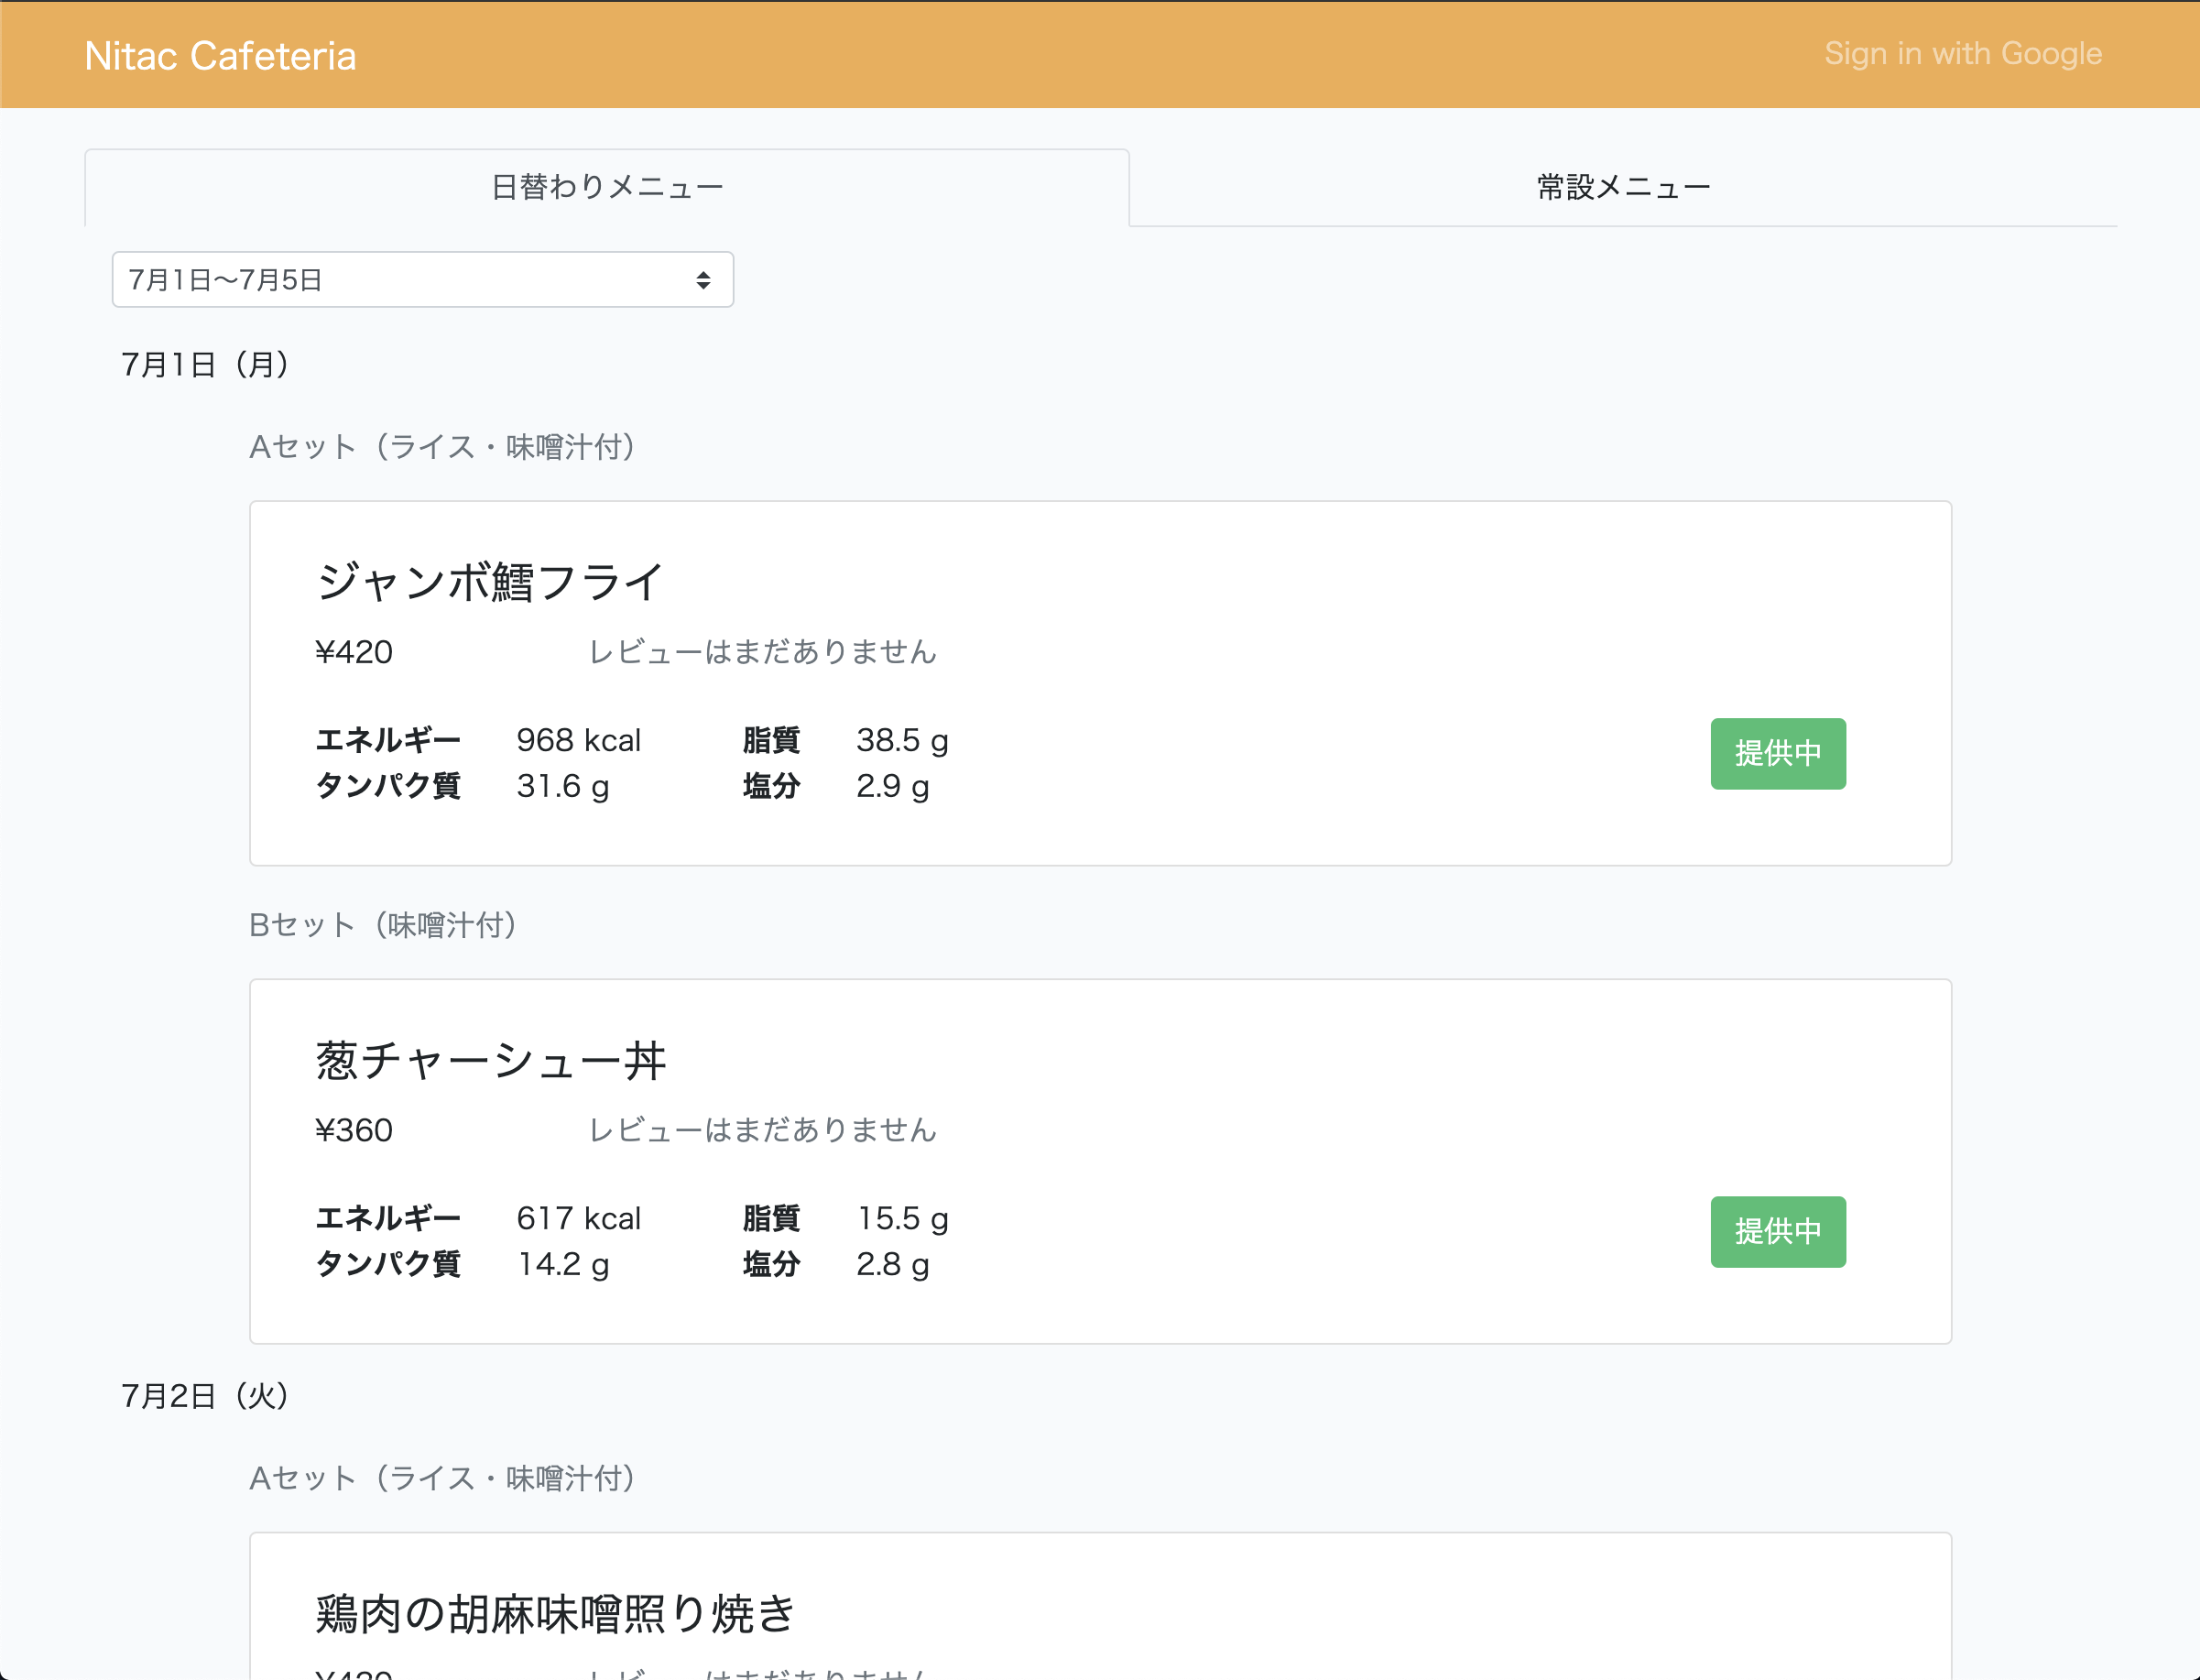
\includegraphics[scale = 0.22525]{image/menu.png}
    \caption{メニュー画面}
\end{figure}
まず最初にメニュー画面が表示されます。メニュー画面は日替りメニュー、常設メニューの二つの画面からなり、画面上部にあるタブで切り替えることができます(上図は日替わりメニューの画面)。日替りメニュー画面の場合、画面左上にある日付を変更することで表示させたい日付のメニューを表示させることができます。
\newpage
\subsection{メニューカード}
\begin{figure}[htbp]
\centering
	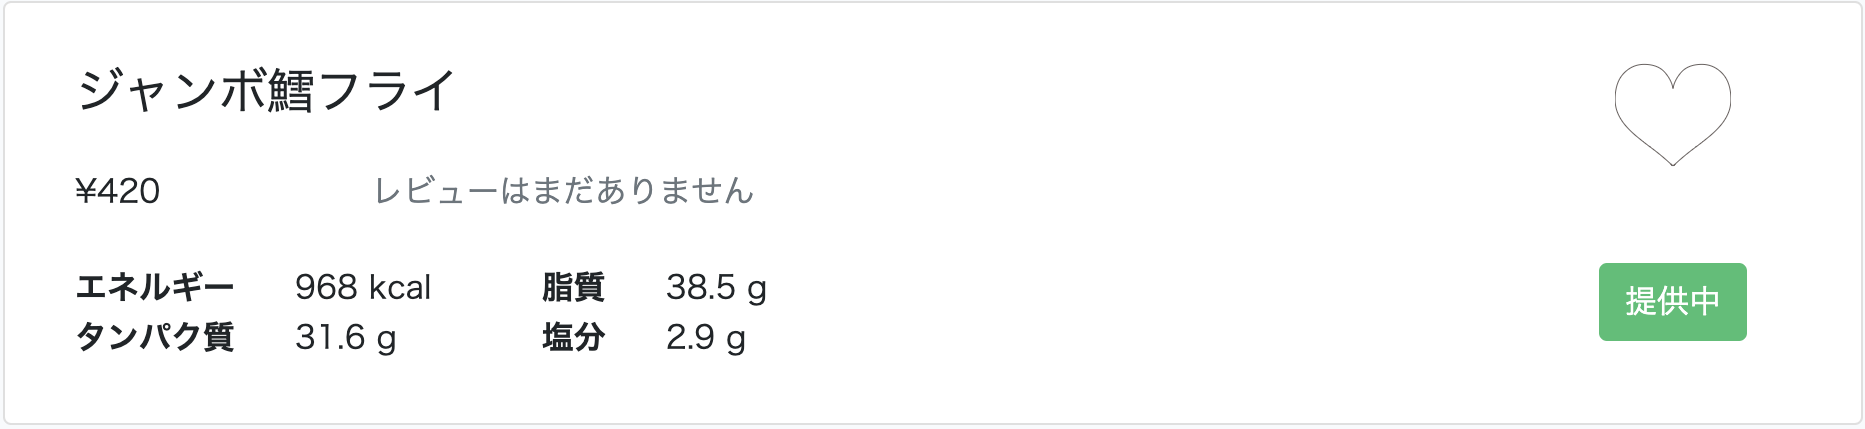
\includegraphics[scale = 0.2]{image/menucard.png}
	\caption{メニューカード}
\end{figure}

メニューカードはそれぞれの料理毎に並べられています。\\
\begin{figure}[htbp]
\centering
	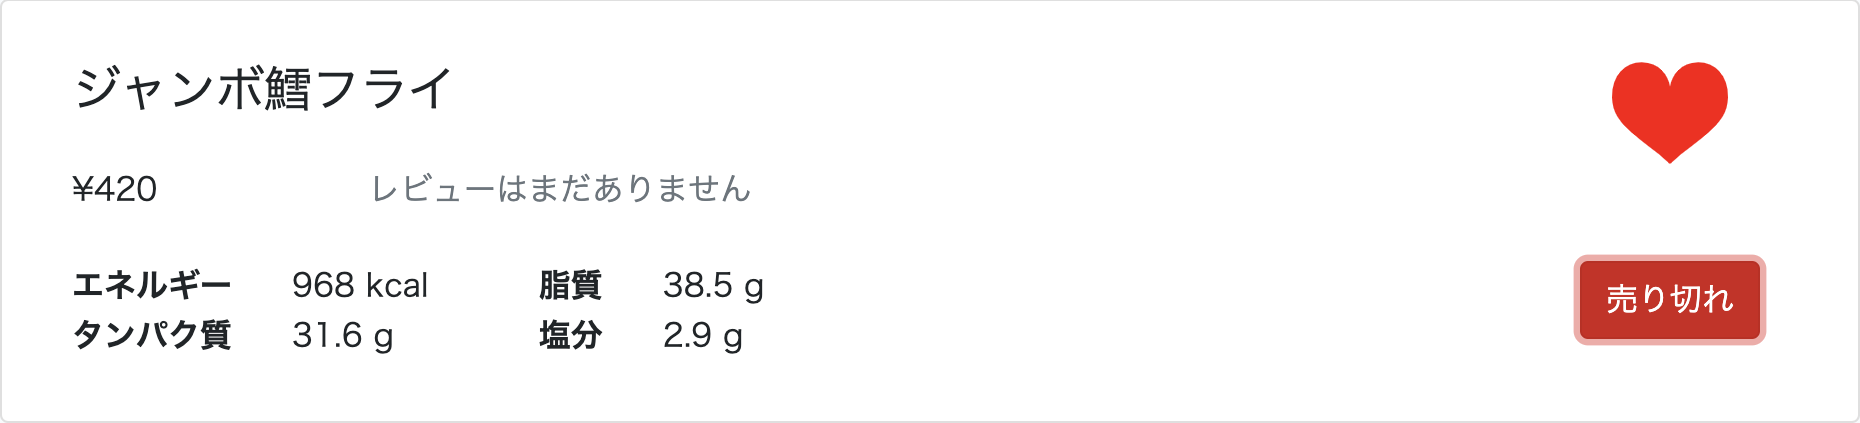
\includegraphics[scale = 0.2]{image/menucard2.png}
	\caption{売り切れの状態およびお気に入り登録済みの状態}
\end{figure}
カード上の提供中というボタンをタップすると、売り切れの状態に変化させることができます。\\
売り切れの状態なら、売り切れというボタンをタップすると提供中の状態に変化させることができます。\\
もしあなたがログインしているならば、ハートマークをタップするとお気に入り登録することができます。またお気に入り登録されたメニューはマイページより確認することができます。\\
メニューカード上のハートマークまたは提供中、売り切れのボタン以外の場所をタップするとメニュー詳細画面に遷移します。
\newpage
\section{メニュー詳細画面}
\begin{figure}[htbp]
\centering
	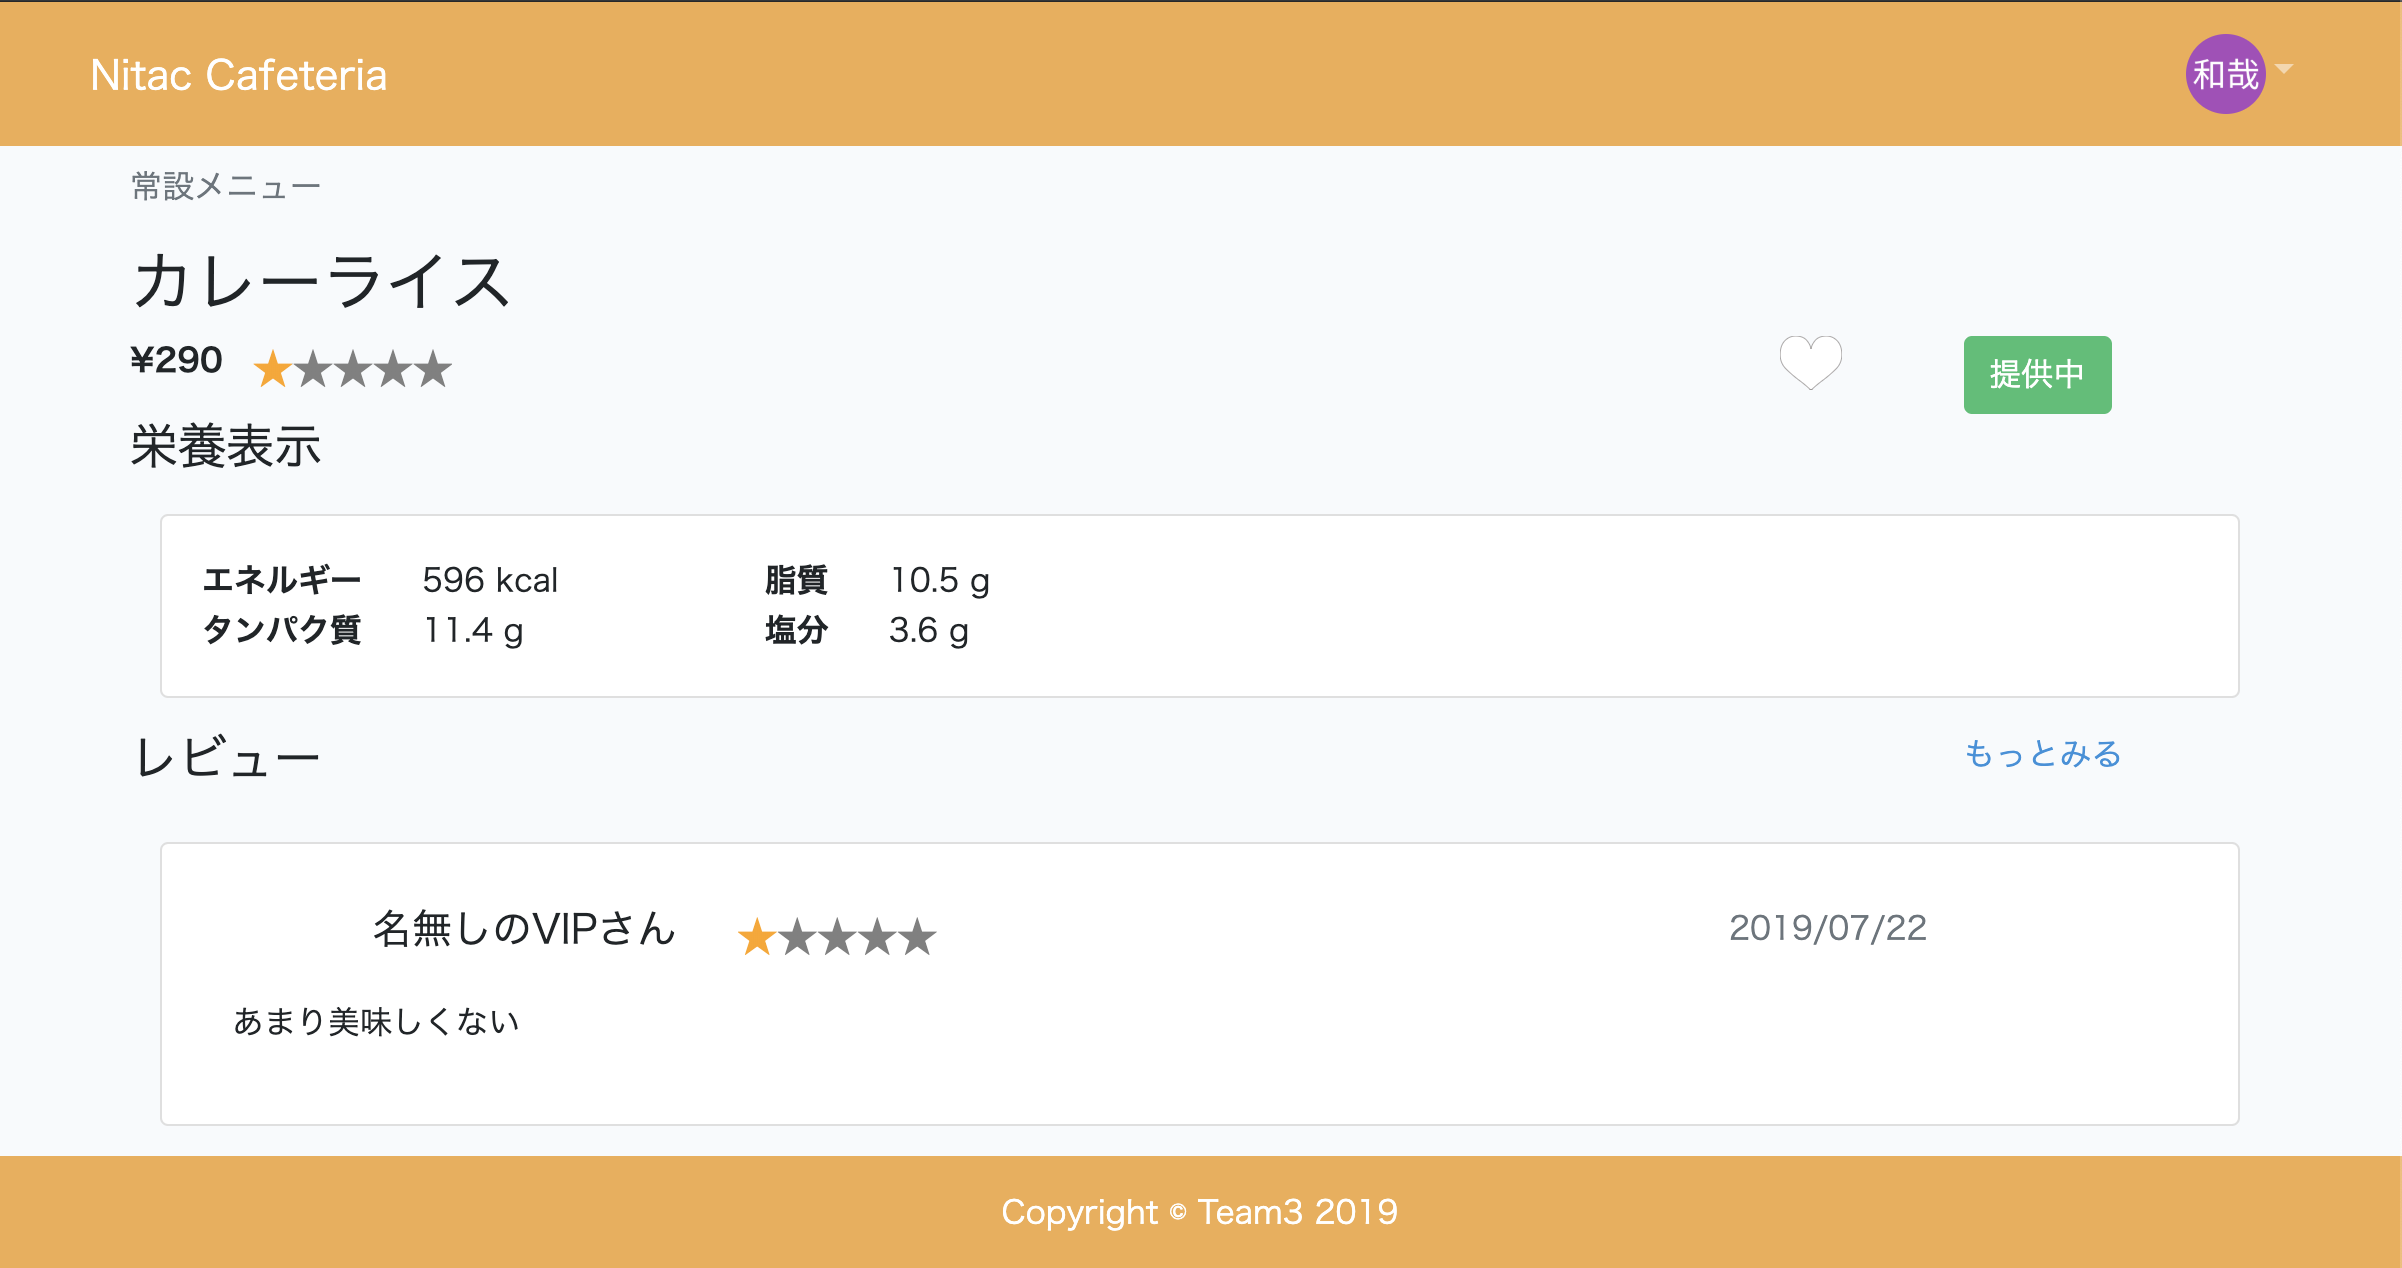
\includegraphics[scale = 0.225]{image/detail.png}
	\caption{メニュー詳細画面}
\end{figure}
メニュー詳細画面では他のユーザーが投稿したメニューの画像及びレビュー等を閲覧することができます。\\
ここでも提供中または売り切れのボタンをタップすることでその状態を変化させることができます。\\
画面右中部にある「もっと見る」をタップすることによって、レビュー一覧画面に遷移することができます。\\
\subsection{レビュー一覧画面}
\begin{figure}[htbp]
\centering
	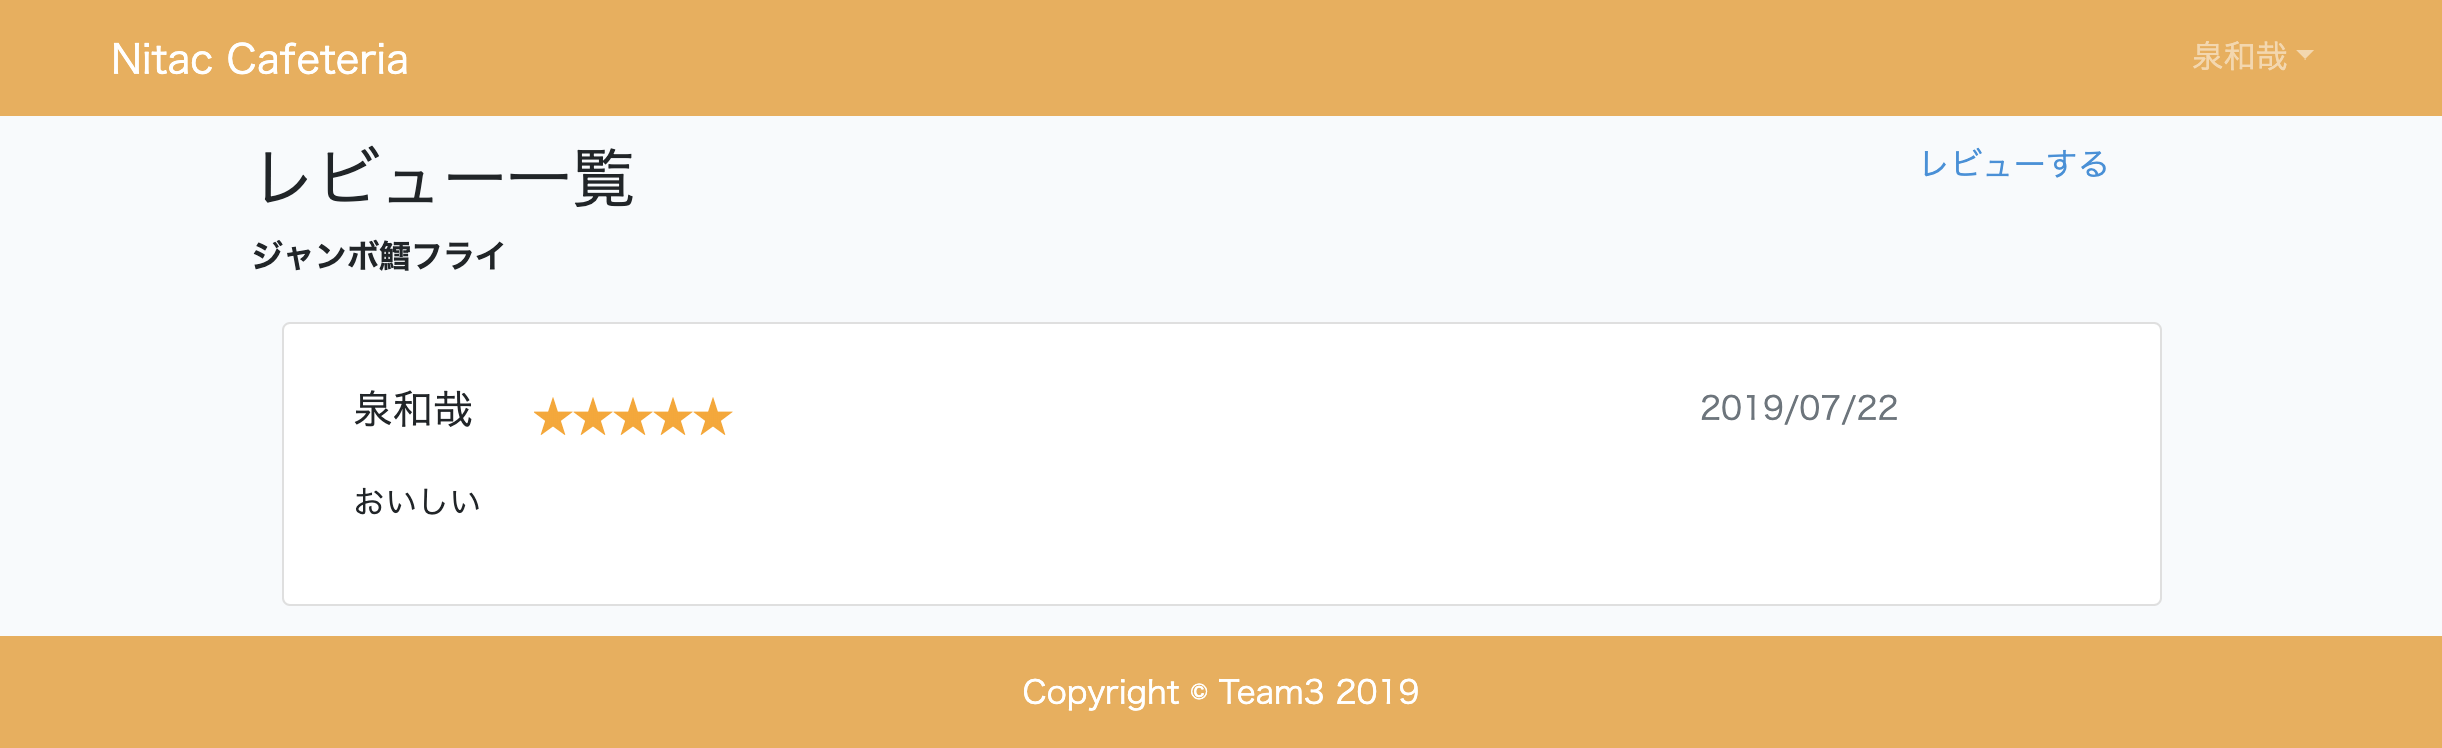
\includegraphics[scale = 0.225]{image/review.png}
	\caption{レビュー一覧画面}
\end{figure}
レビュー一覧画面では、全てのユーザーのレビューを閲覧することができます。\\
また、画面右上部にある「レビューする」をタップするとレビュー画面に遷移することができます。
但し、ログインした状態でなければ「レビューをする」が表示されずレビューをすることは出来ません。\\
\newpage
\subsection{レビュー画面(ログイン時のみ)}
\begin{figure}[htbp]
\centering
	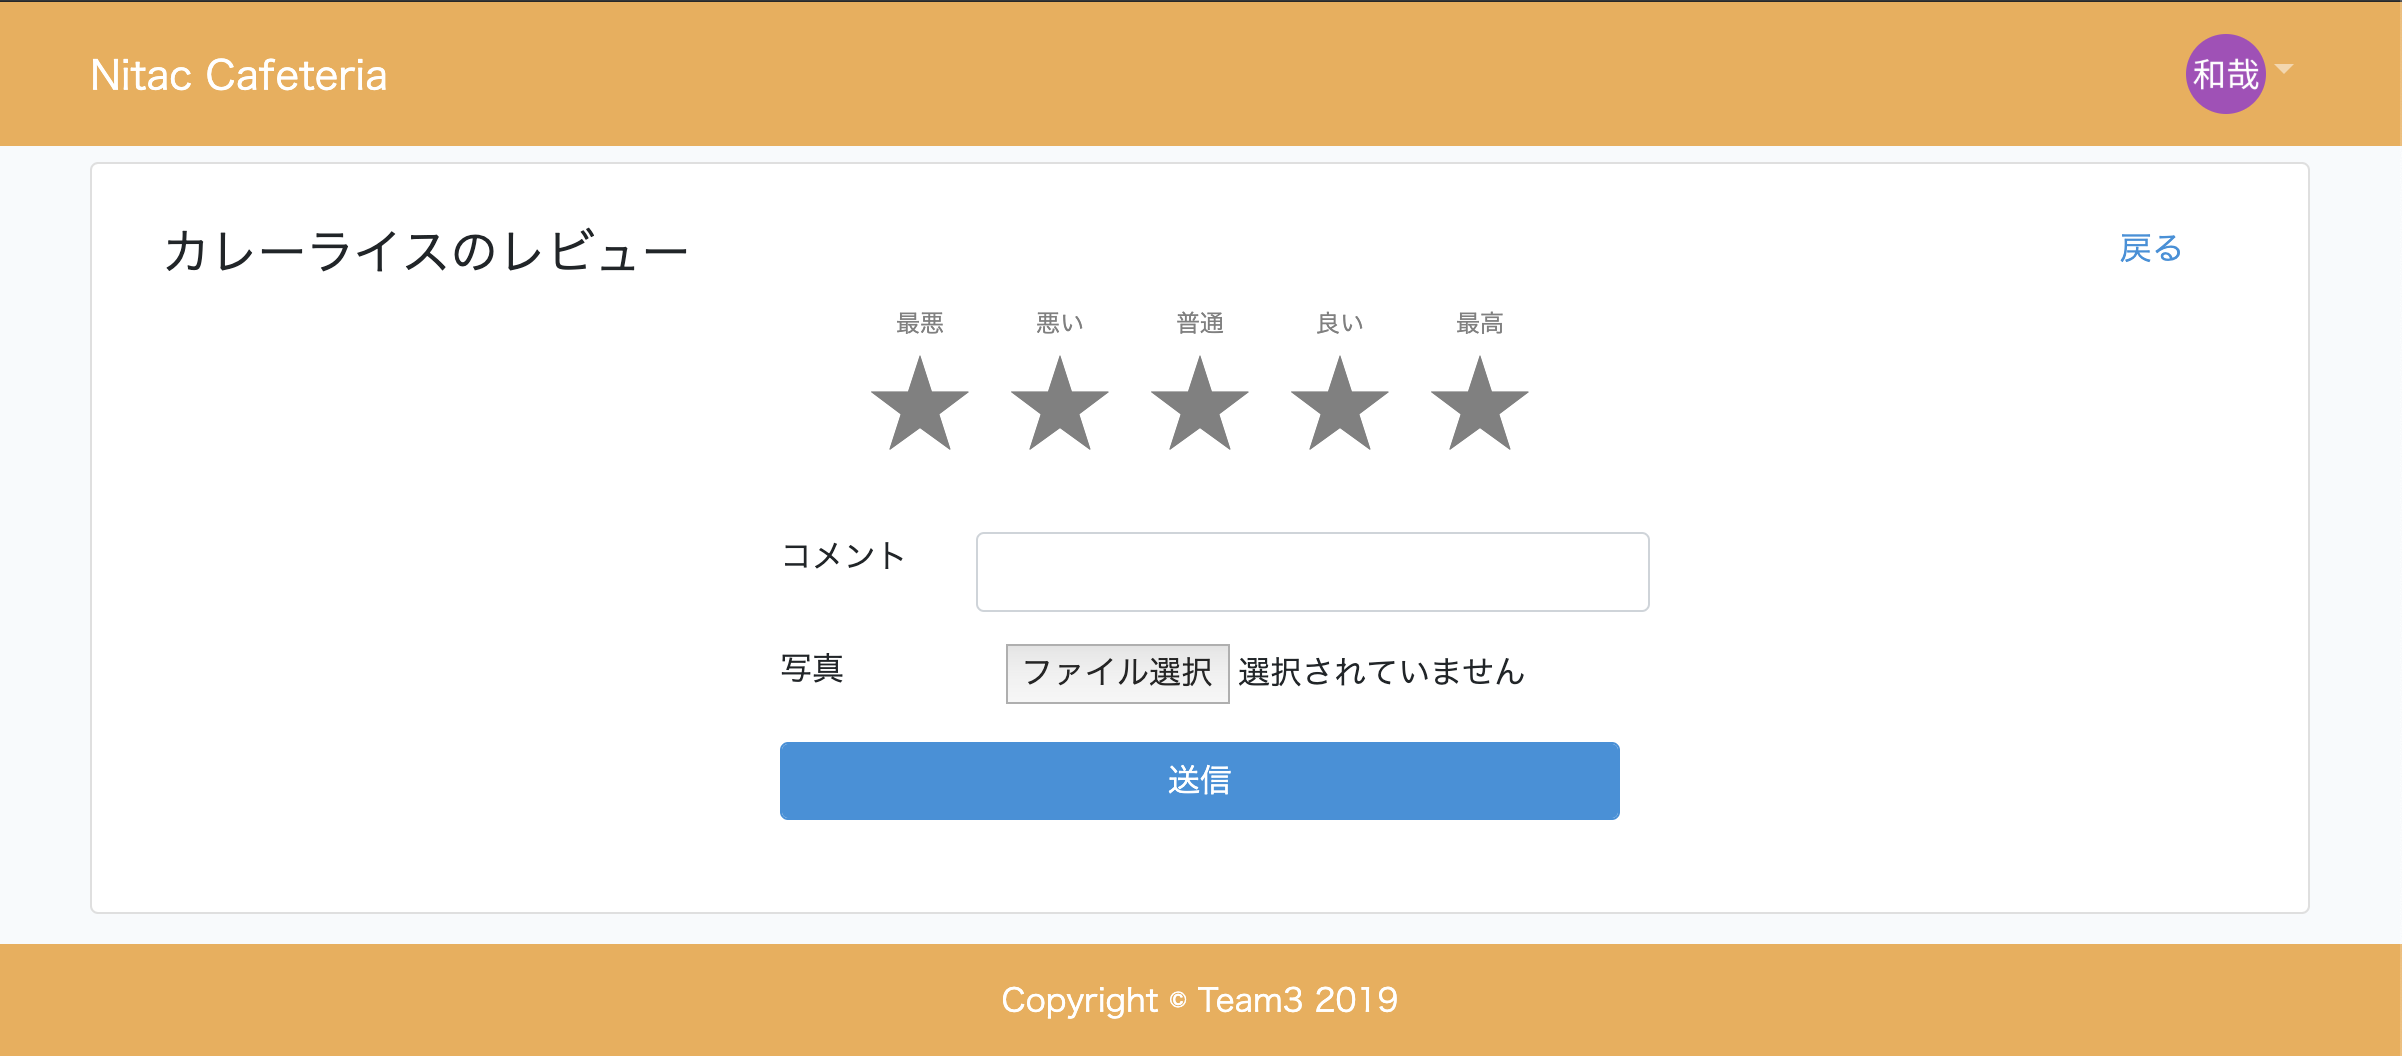
\includegraphics[scale = 0.225]{image/review2.png}
	\caption{レビュー画面}
\end{figure}
レビュー画面ではメニューを五段階評価(星の数)で評価し、コメント及び写真を投稿することができます。\\
星の数やコメントなどの設定が完了しましたら、送信ボタンをタップしてレビューを投稿してください。\\
投稿された写真はメニュー詳細画面(図4)上部の写真の位置に反映されます。\\
投稿されたレビューは、そのメニューのレビュー一覧画面、マイページから確認することができます。\\
\begin{figure}[htbp]
	\centering
		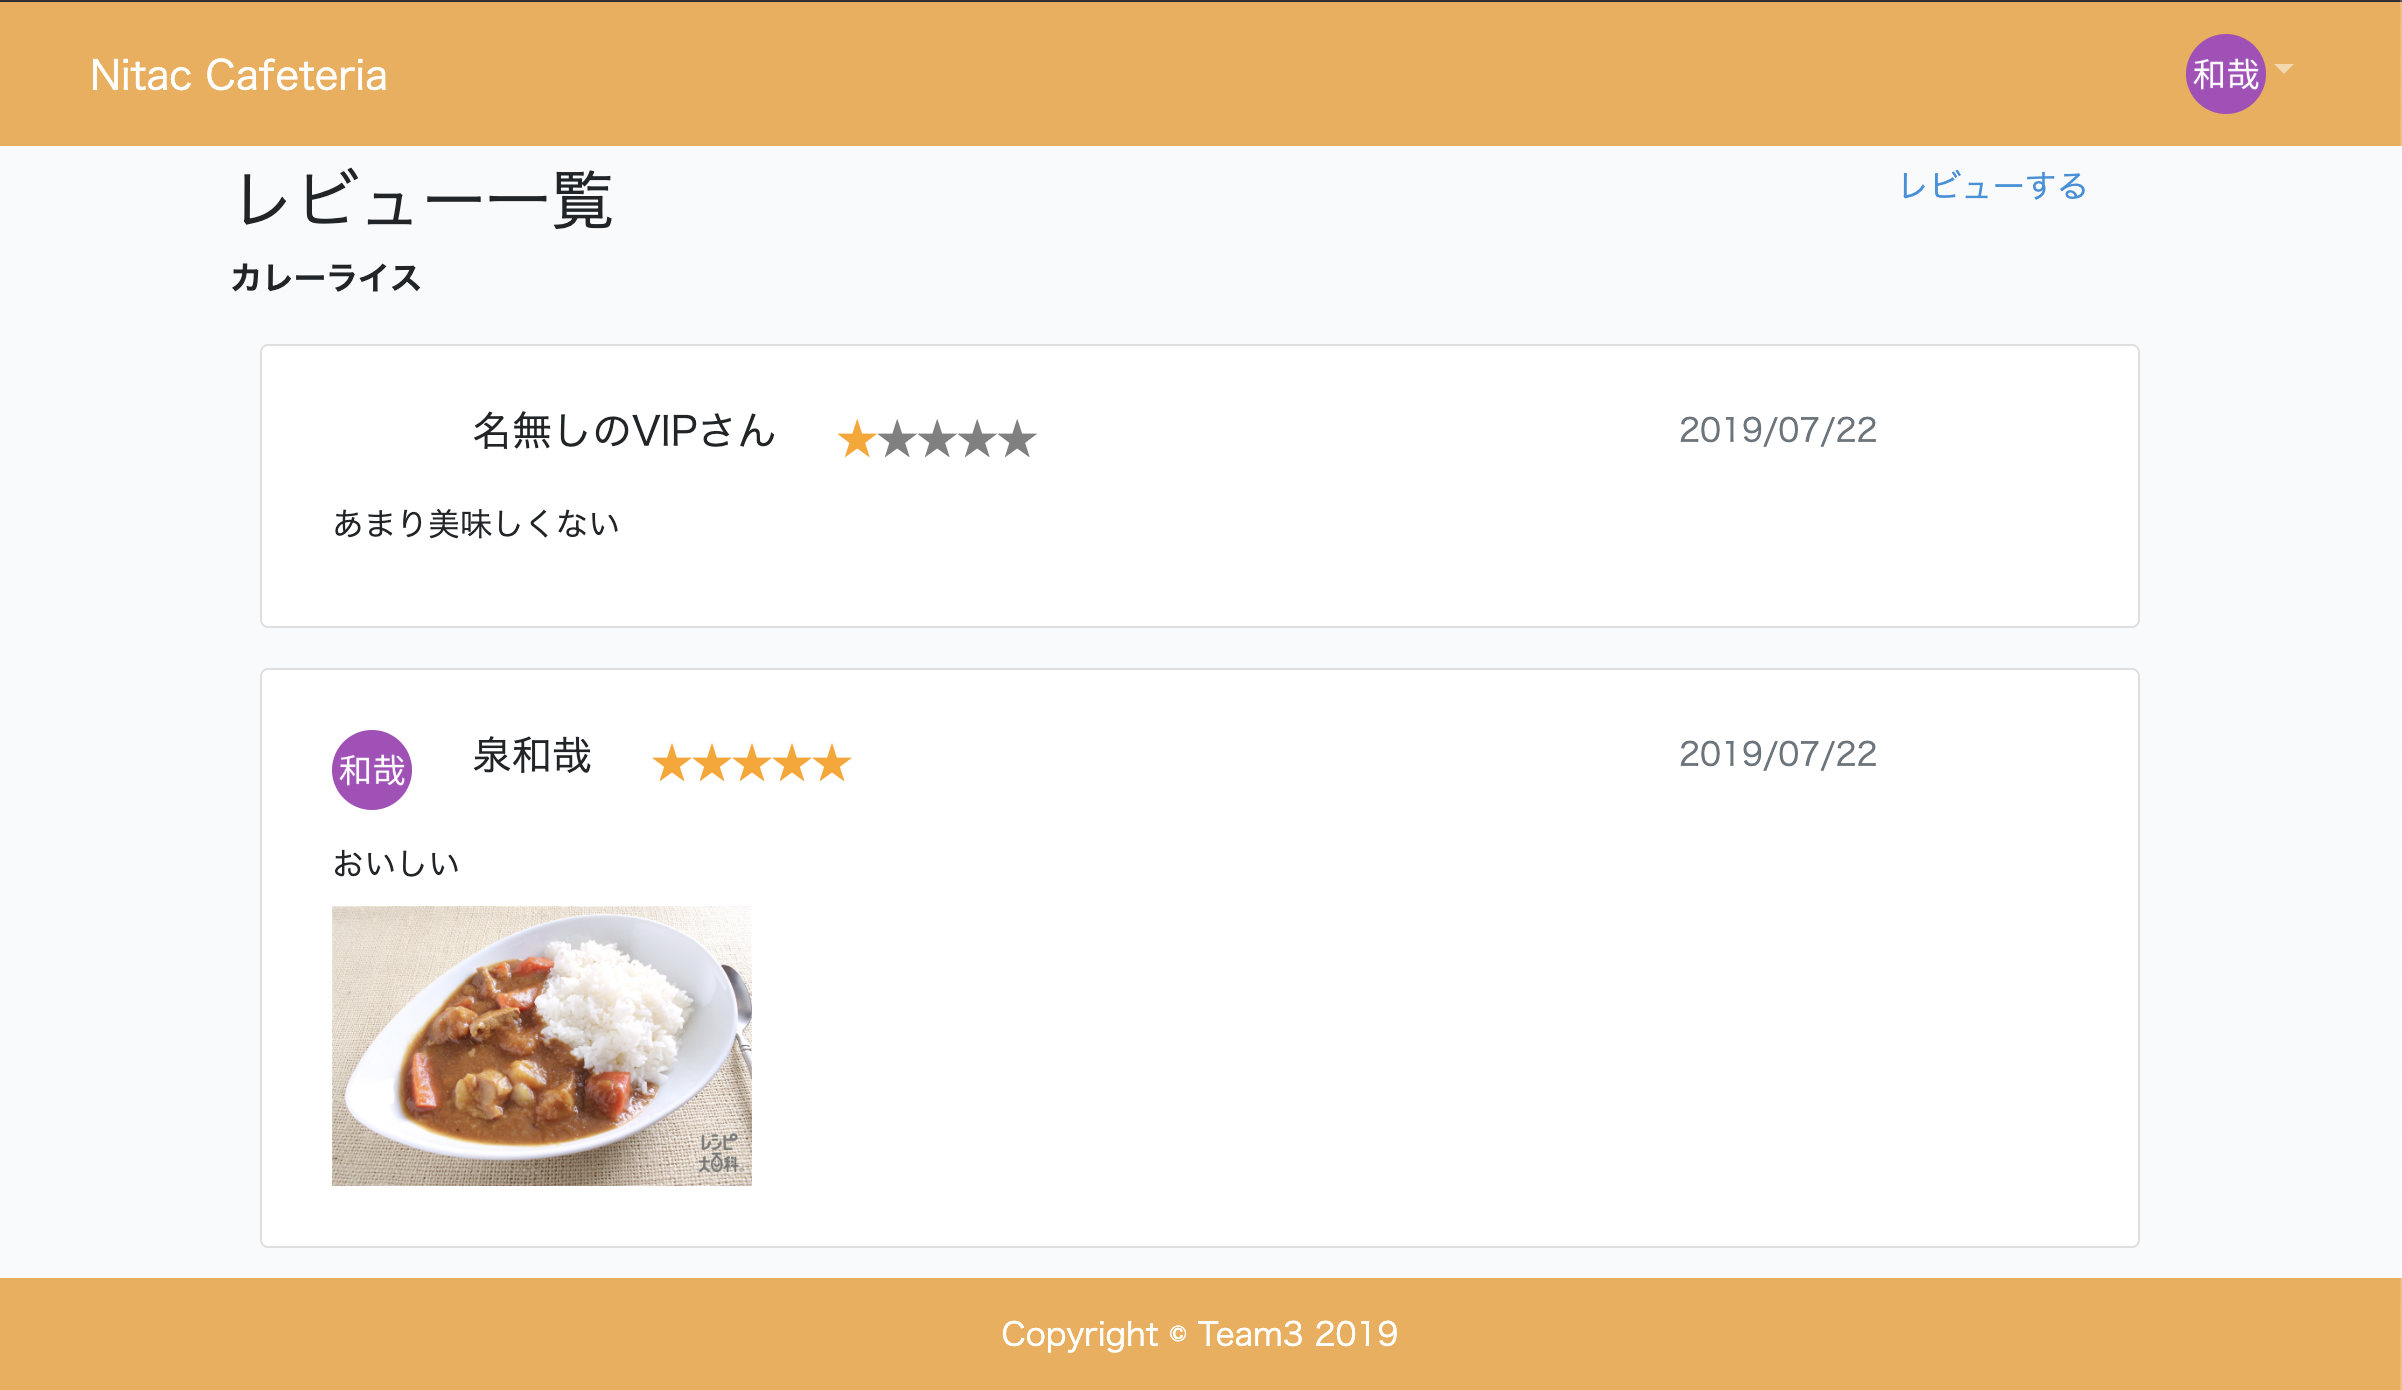
\includegraphics[scale = 0.225]{image/review_after_create.png}
		\caption{レビュー一覧画面(レビュー投稿後)}
	\end{figure}
	\newpage
	\section{ドロップダウンの表示(ログイン時のみ)}
\begin{figure}[htbp]
	\centering
	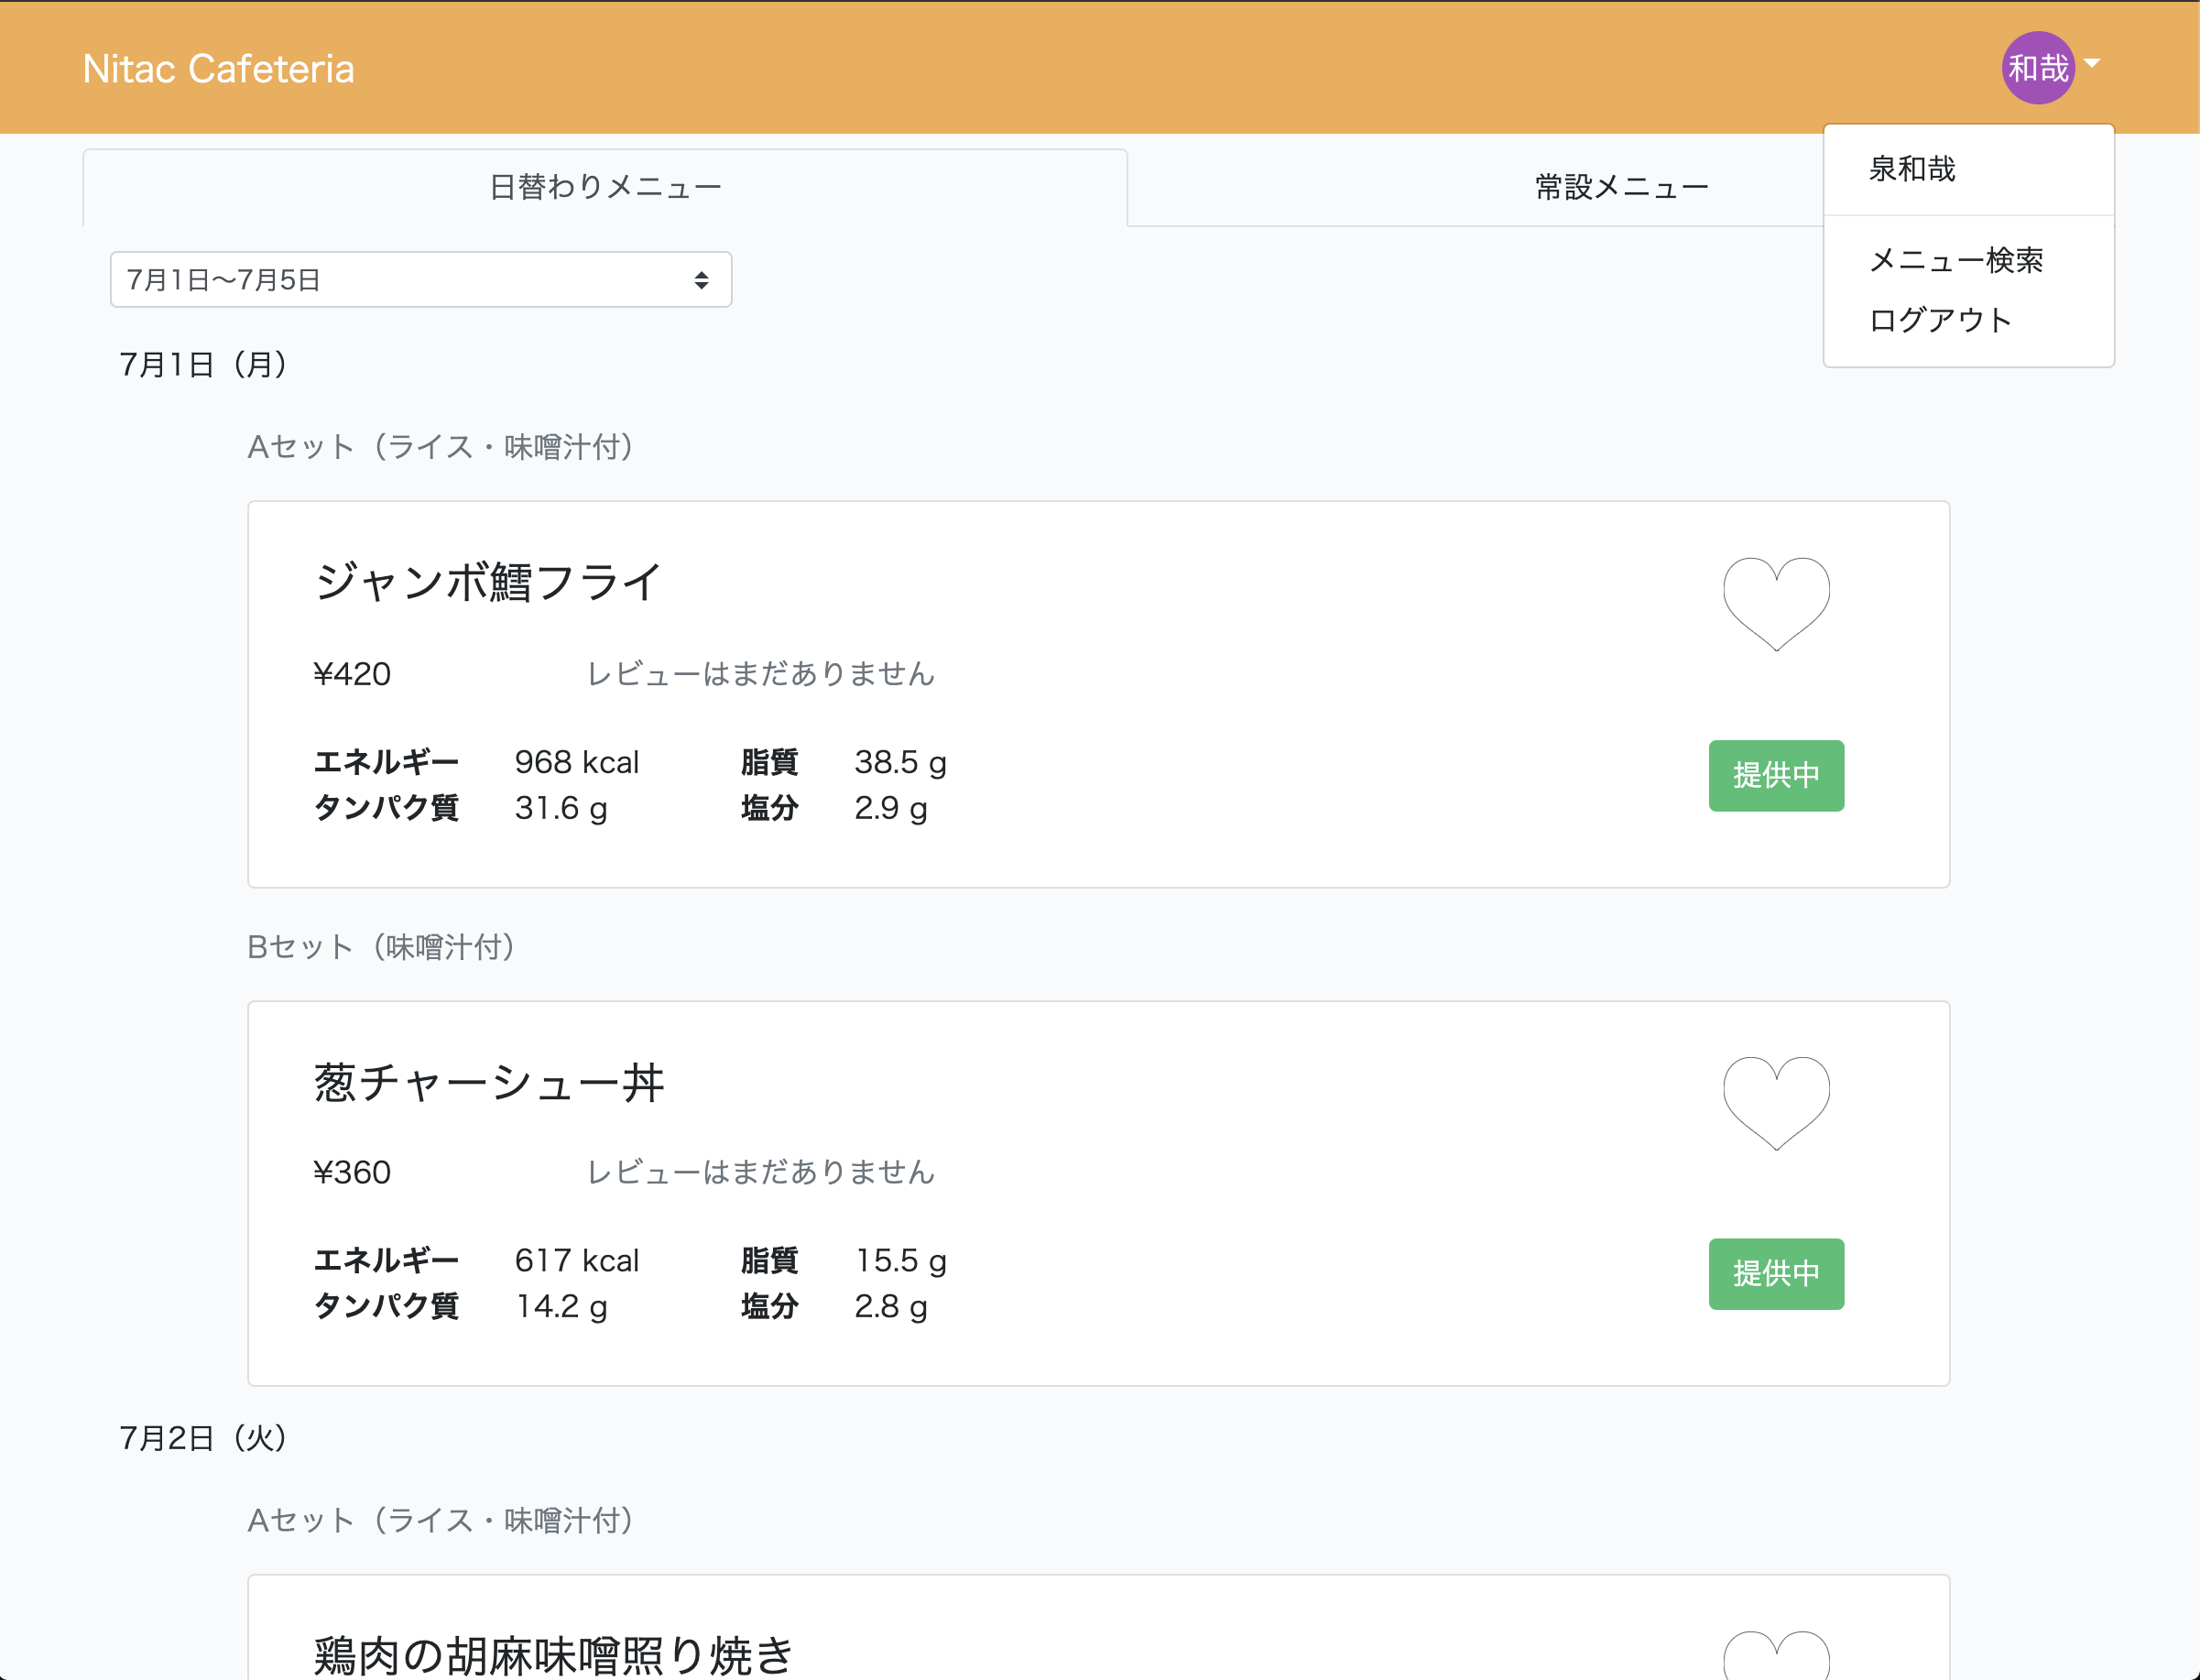
\includegraphics[scale = 0.22525]{image/dropdown_student.png}
	\caption{ドロップダウンの表示}
\end{figure}
画面右上のアイコンをタップすると、ドロップダウンが表示されます。\\
ドロップダウンからはマイページ、メニュー検索、ログアウトに遷移することができます。
\section{マイページ(ログイン時のみ)}
\begin{figure}[htbp]
\centering
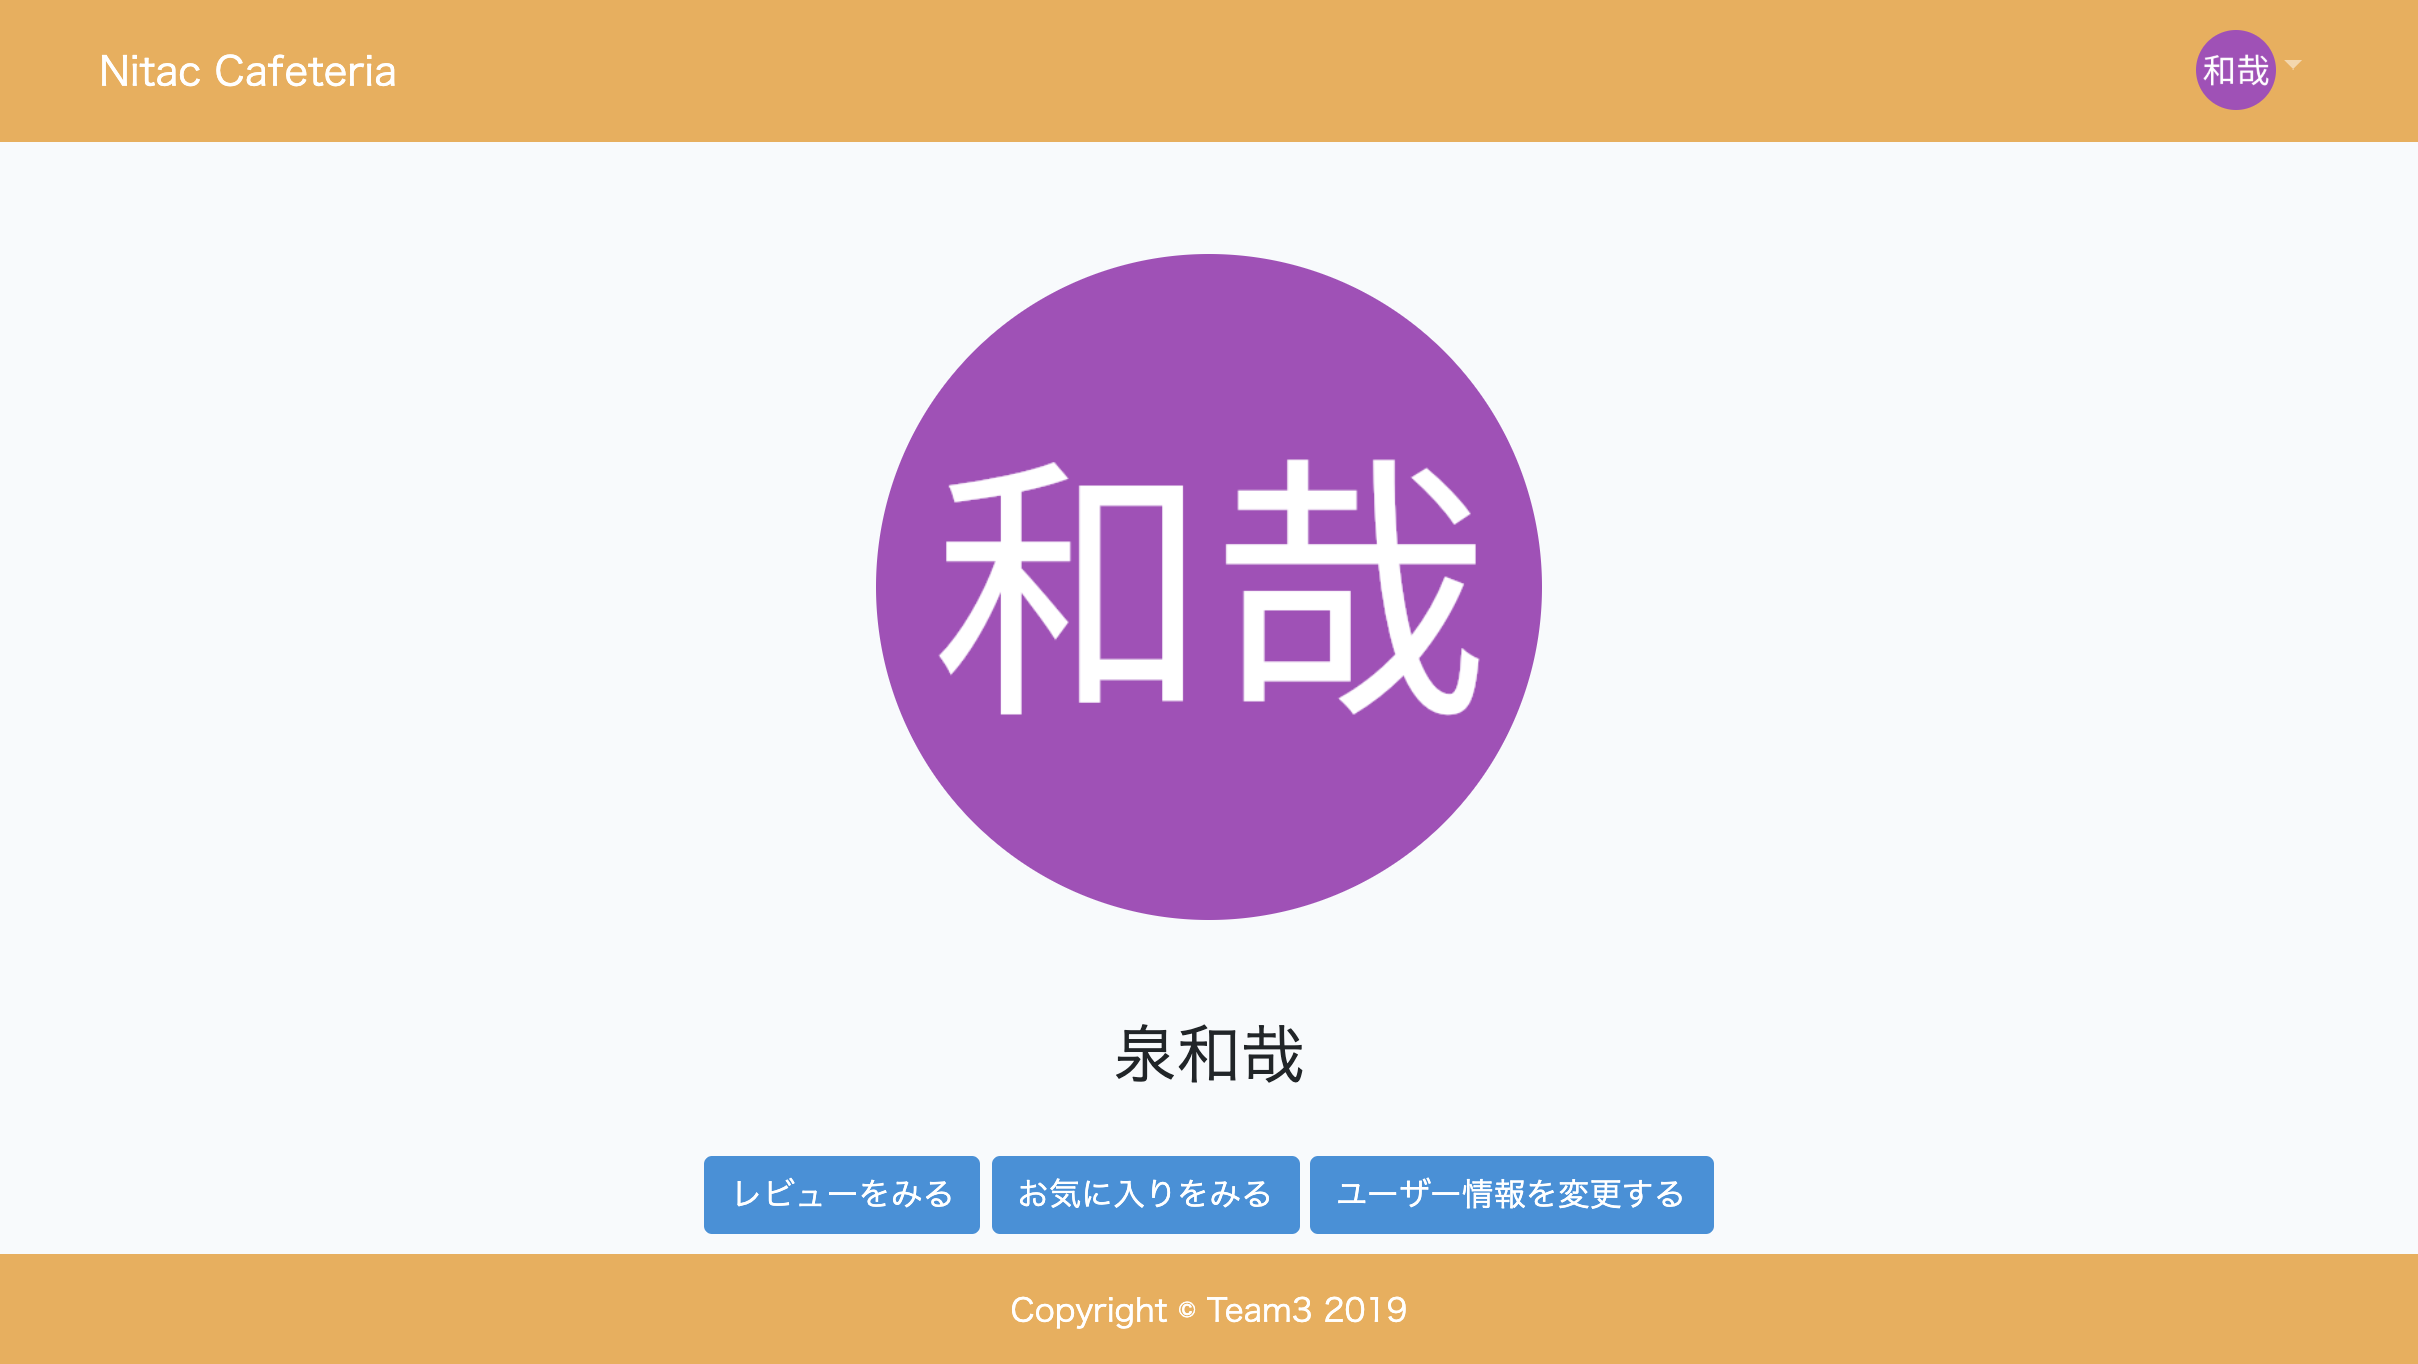
\includegraphics[scale = 0.225]{image/mypage.png}
\caption{マイページ画面}
\end{figure}
画面右上のアイコンをタップして、表示されたドロップダウンの中にあるユーザー名をタップすると、マイページに遷移します。\\
マイページからはユーザー情報変更画面、レビュー一覧画面、お気に入り一覧画面に遷移することができます。
\subsection{マイページ・ユーザー情報変更画面}
\begin{figure}[htbp]
	\centering
	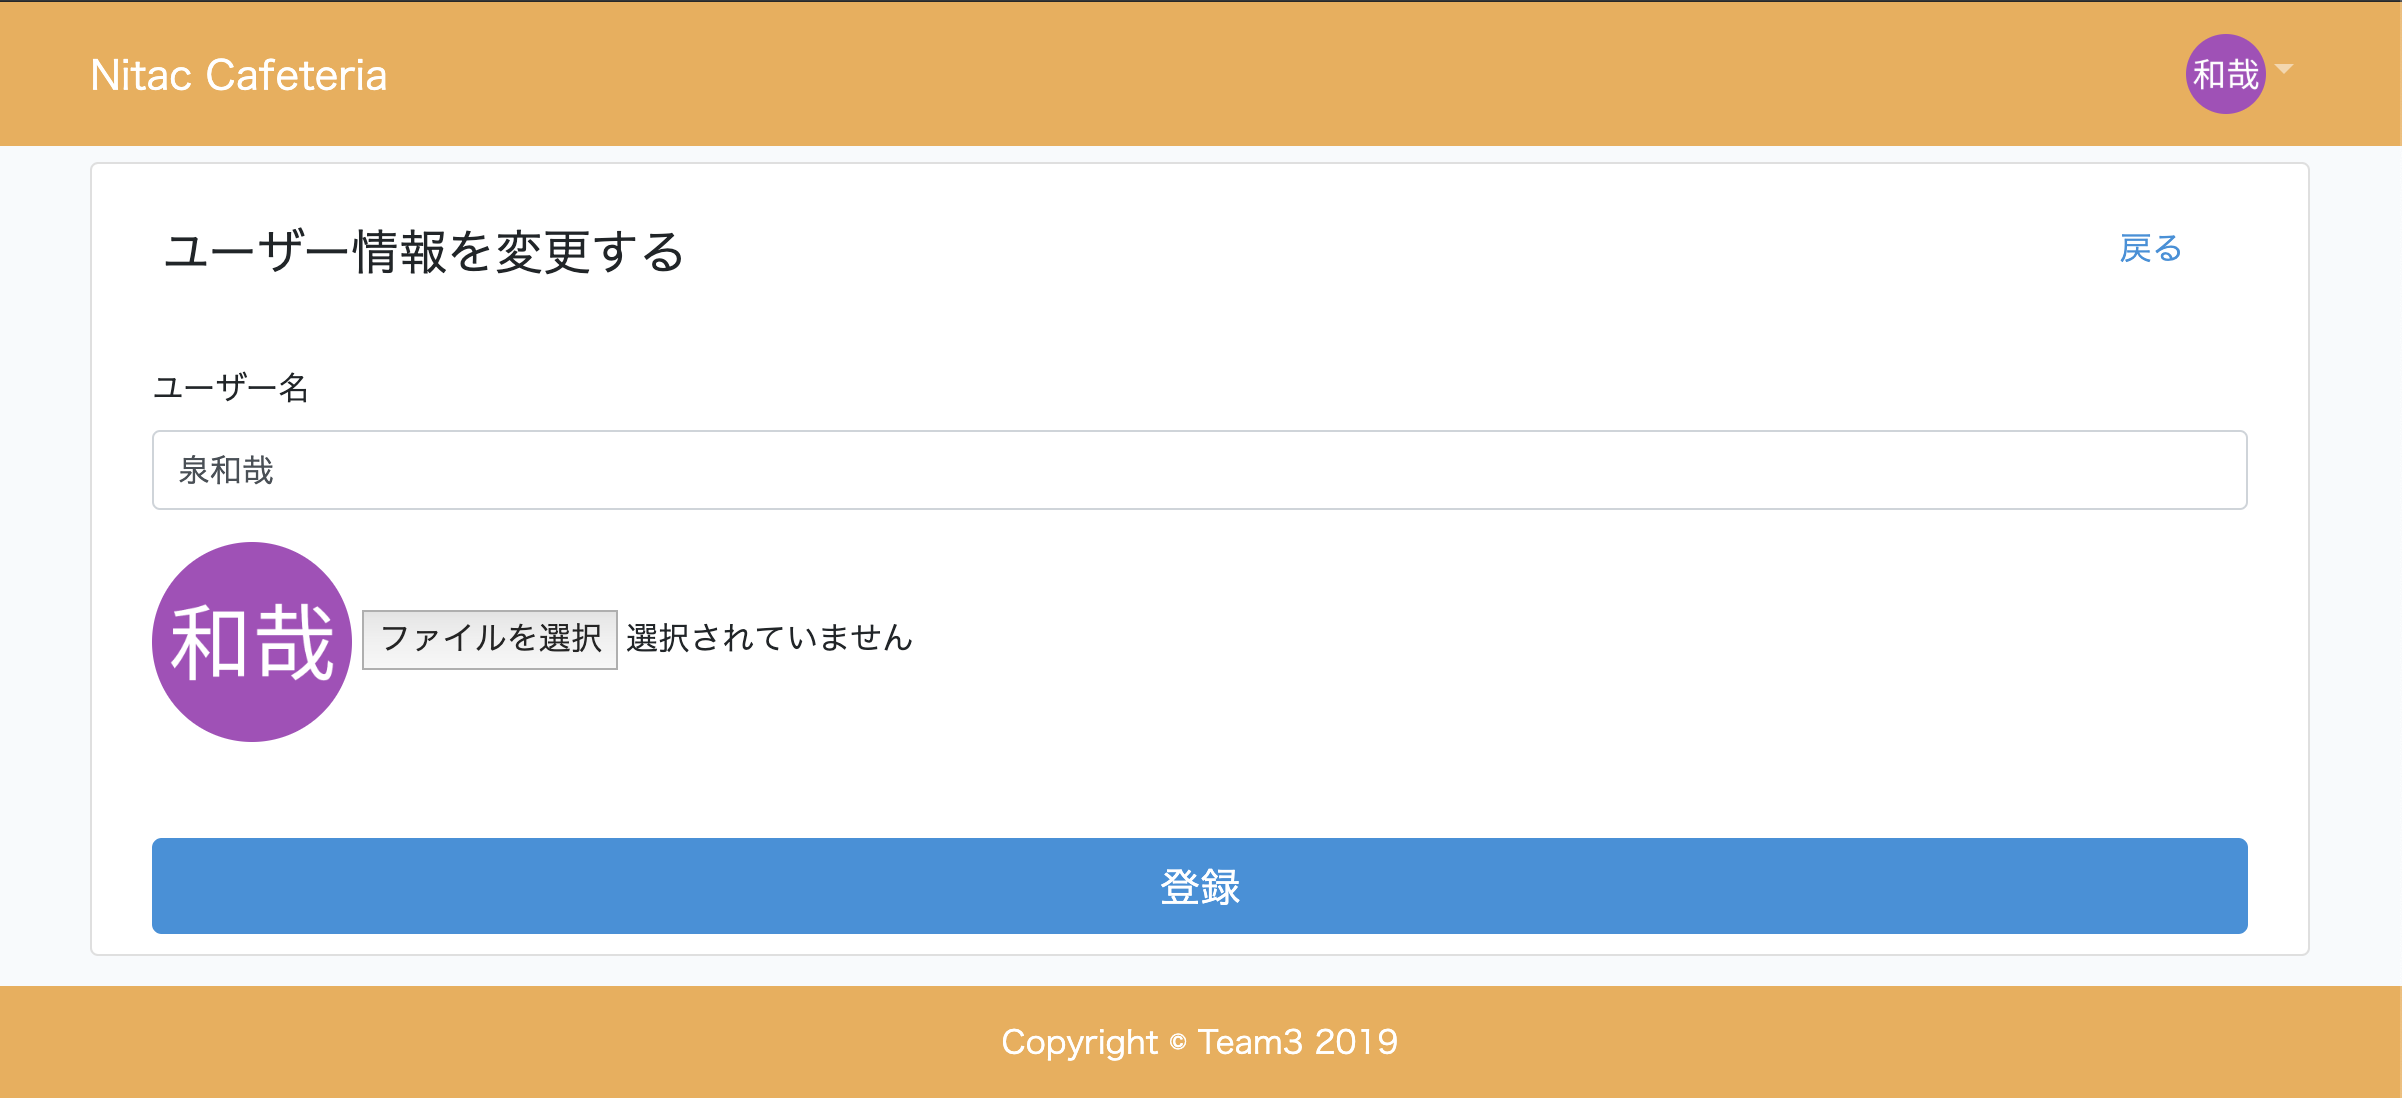
\includegraphics[scale = 0.225]{image/edit_user.png}
	\caption{マイページ・ユーザー情報変更画面}
\end{figure}
この画面ではユーザー名やアイコンを変更することができます。
\subsection{マイページ・レビュー一覧画面}
\begin{figure}[htbp]
\centering
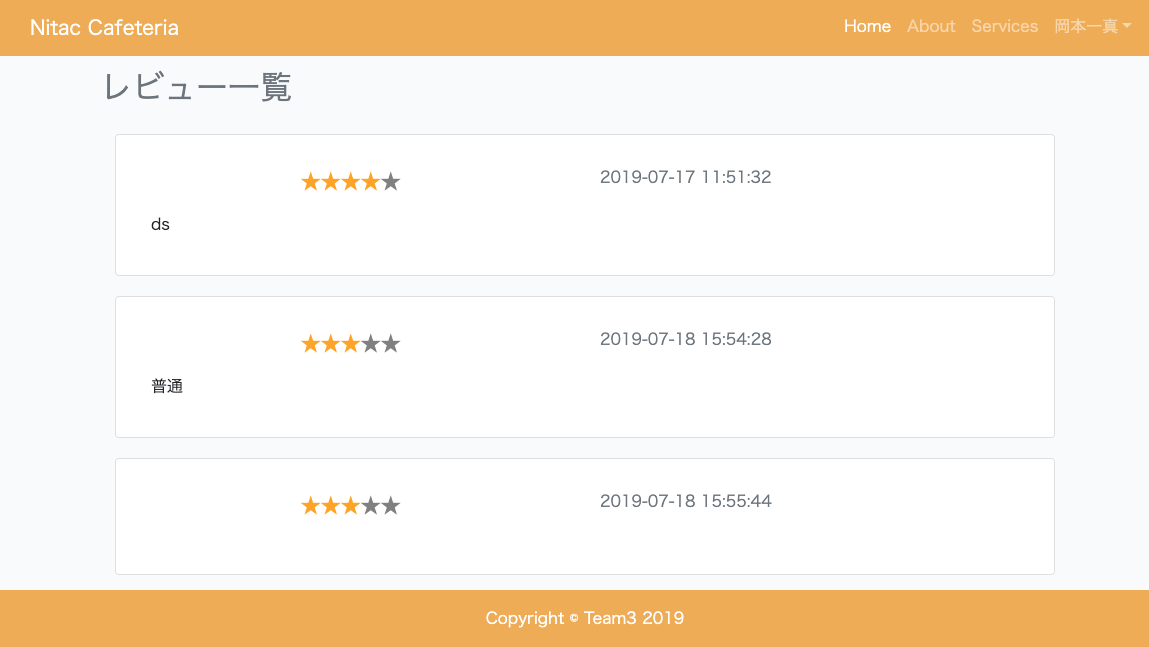
\includegraphics[scale = 0.225]{image/myreview.png}
\caption{マイページ・レビュー一覧画面}
\end{figure}
この画面では今までに投稿したレビューを確認することができます。
\newpage
\subsection{マイページ・お気に入り一覧画面}
\begin{figure}[htbp]
\centering
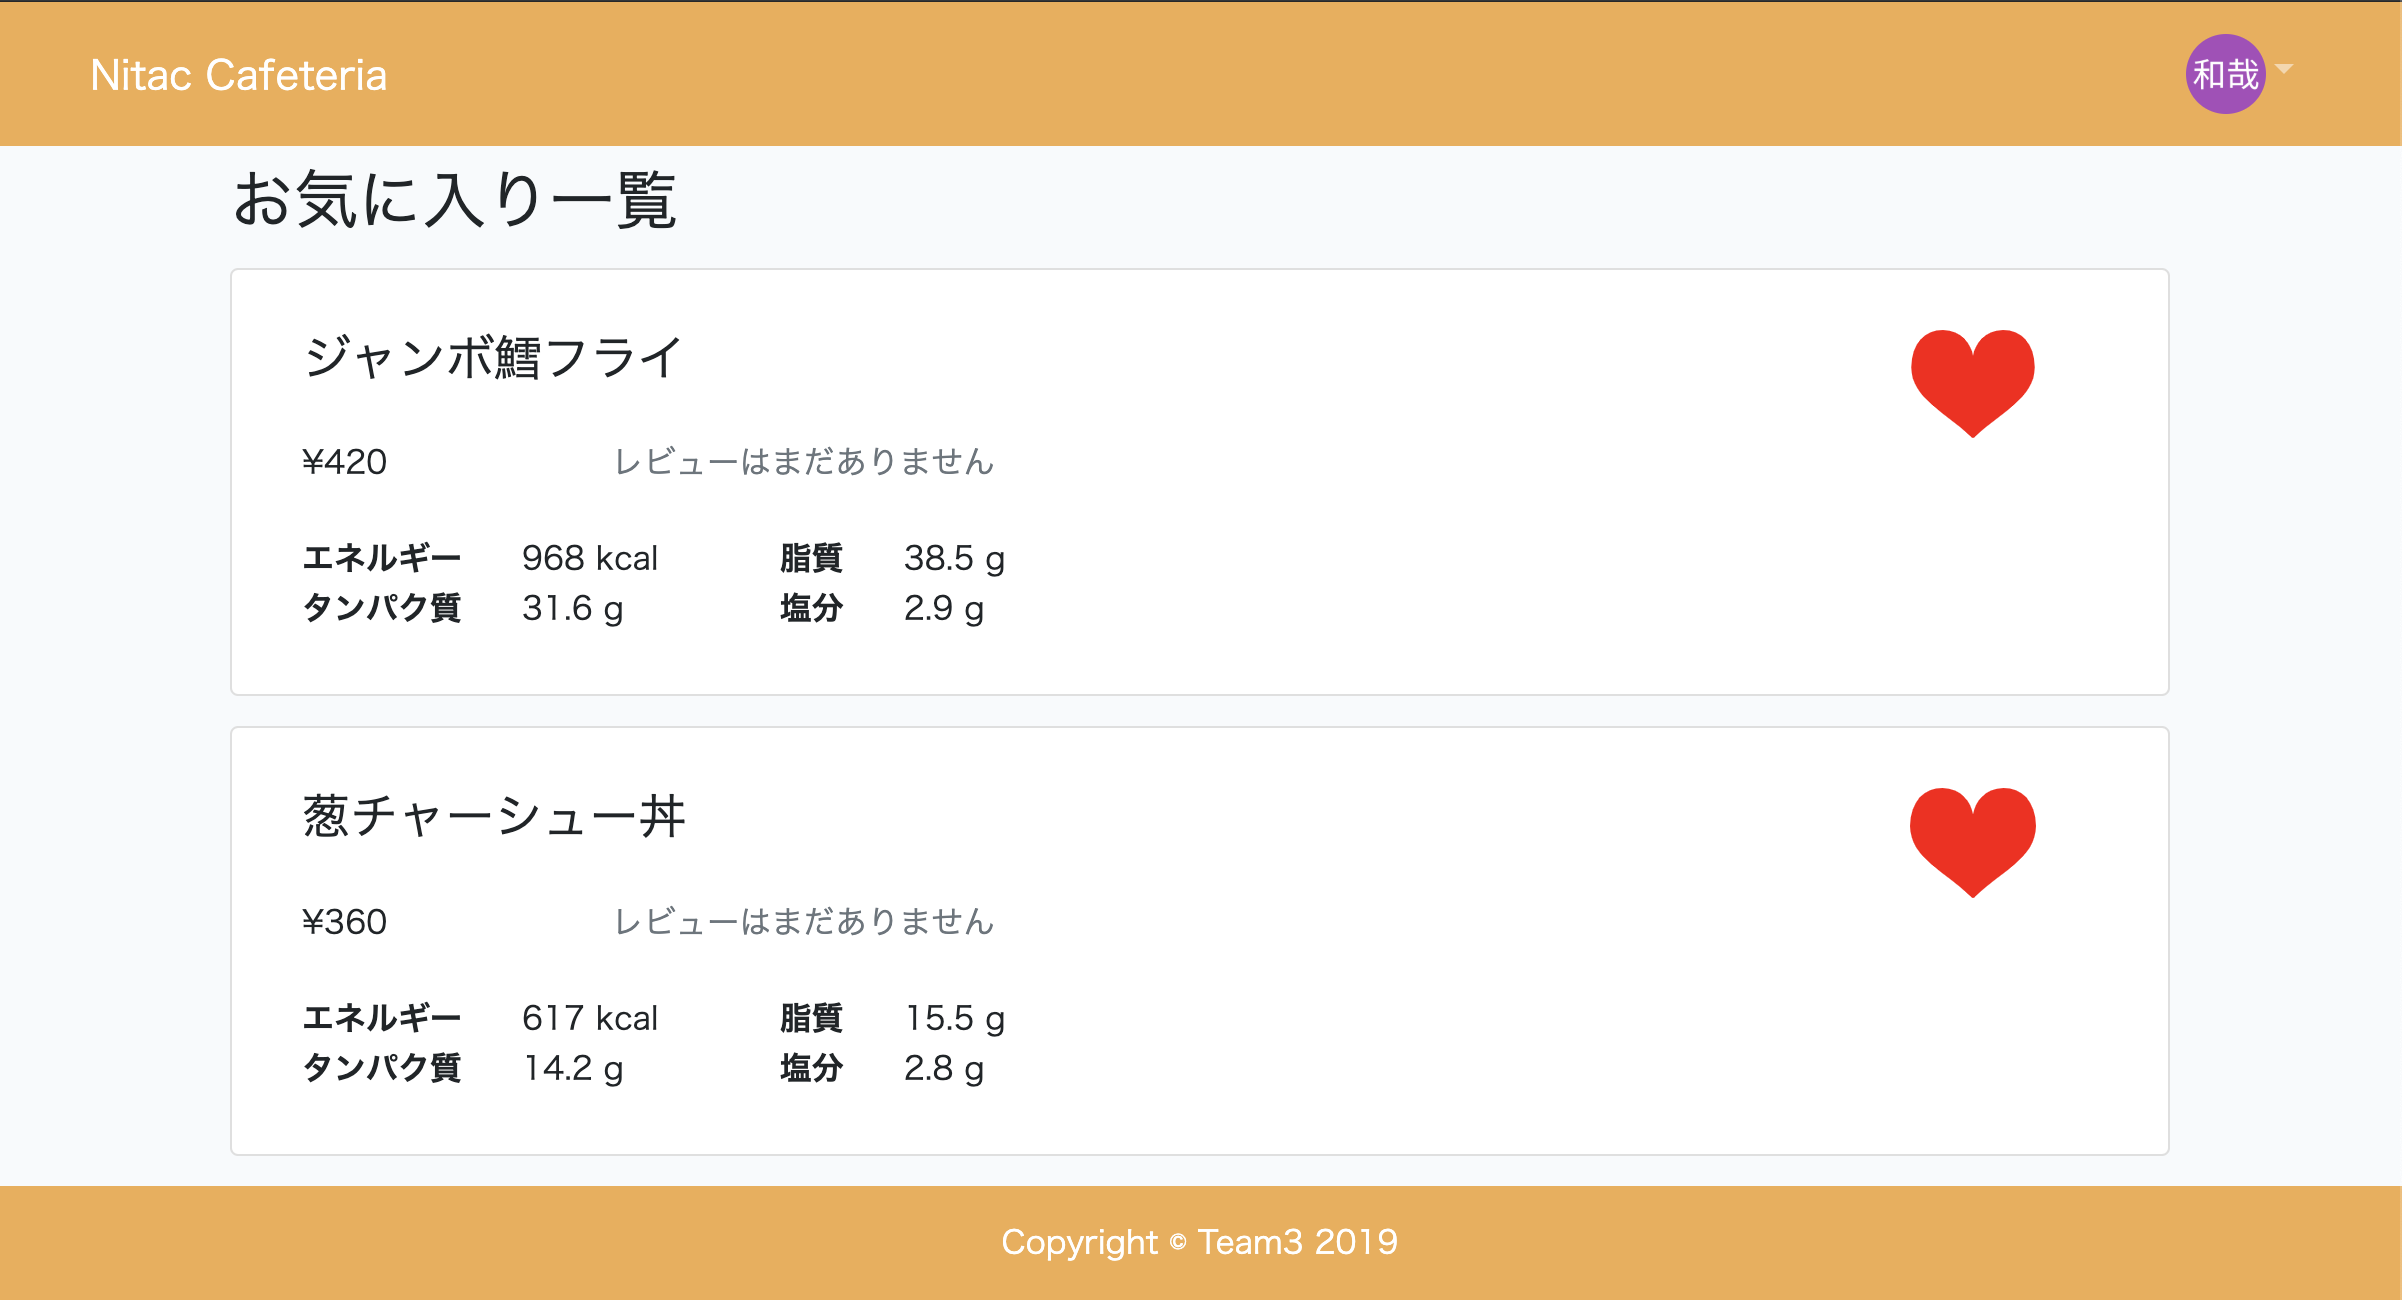
\includegraphics[scale = 0.225]{image/myfavorite.png}
\caption{マイページ・お気に入り一覧画面}
\end{figure}
この画面では今までにお気に入り登録したメニューを確認することができます。
\newpage
\section{管理者用画面(管理者ログイン時)}
\subsection{メニュー画面}
\begin{figure}[htbp]
	\centering
	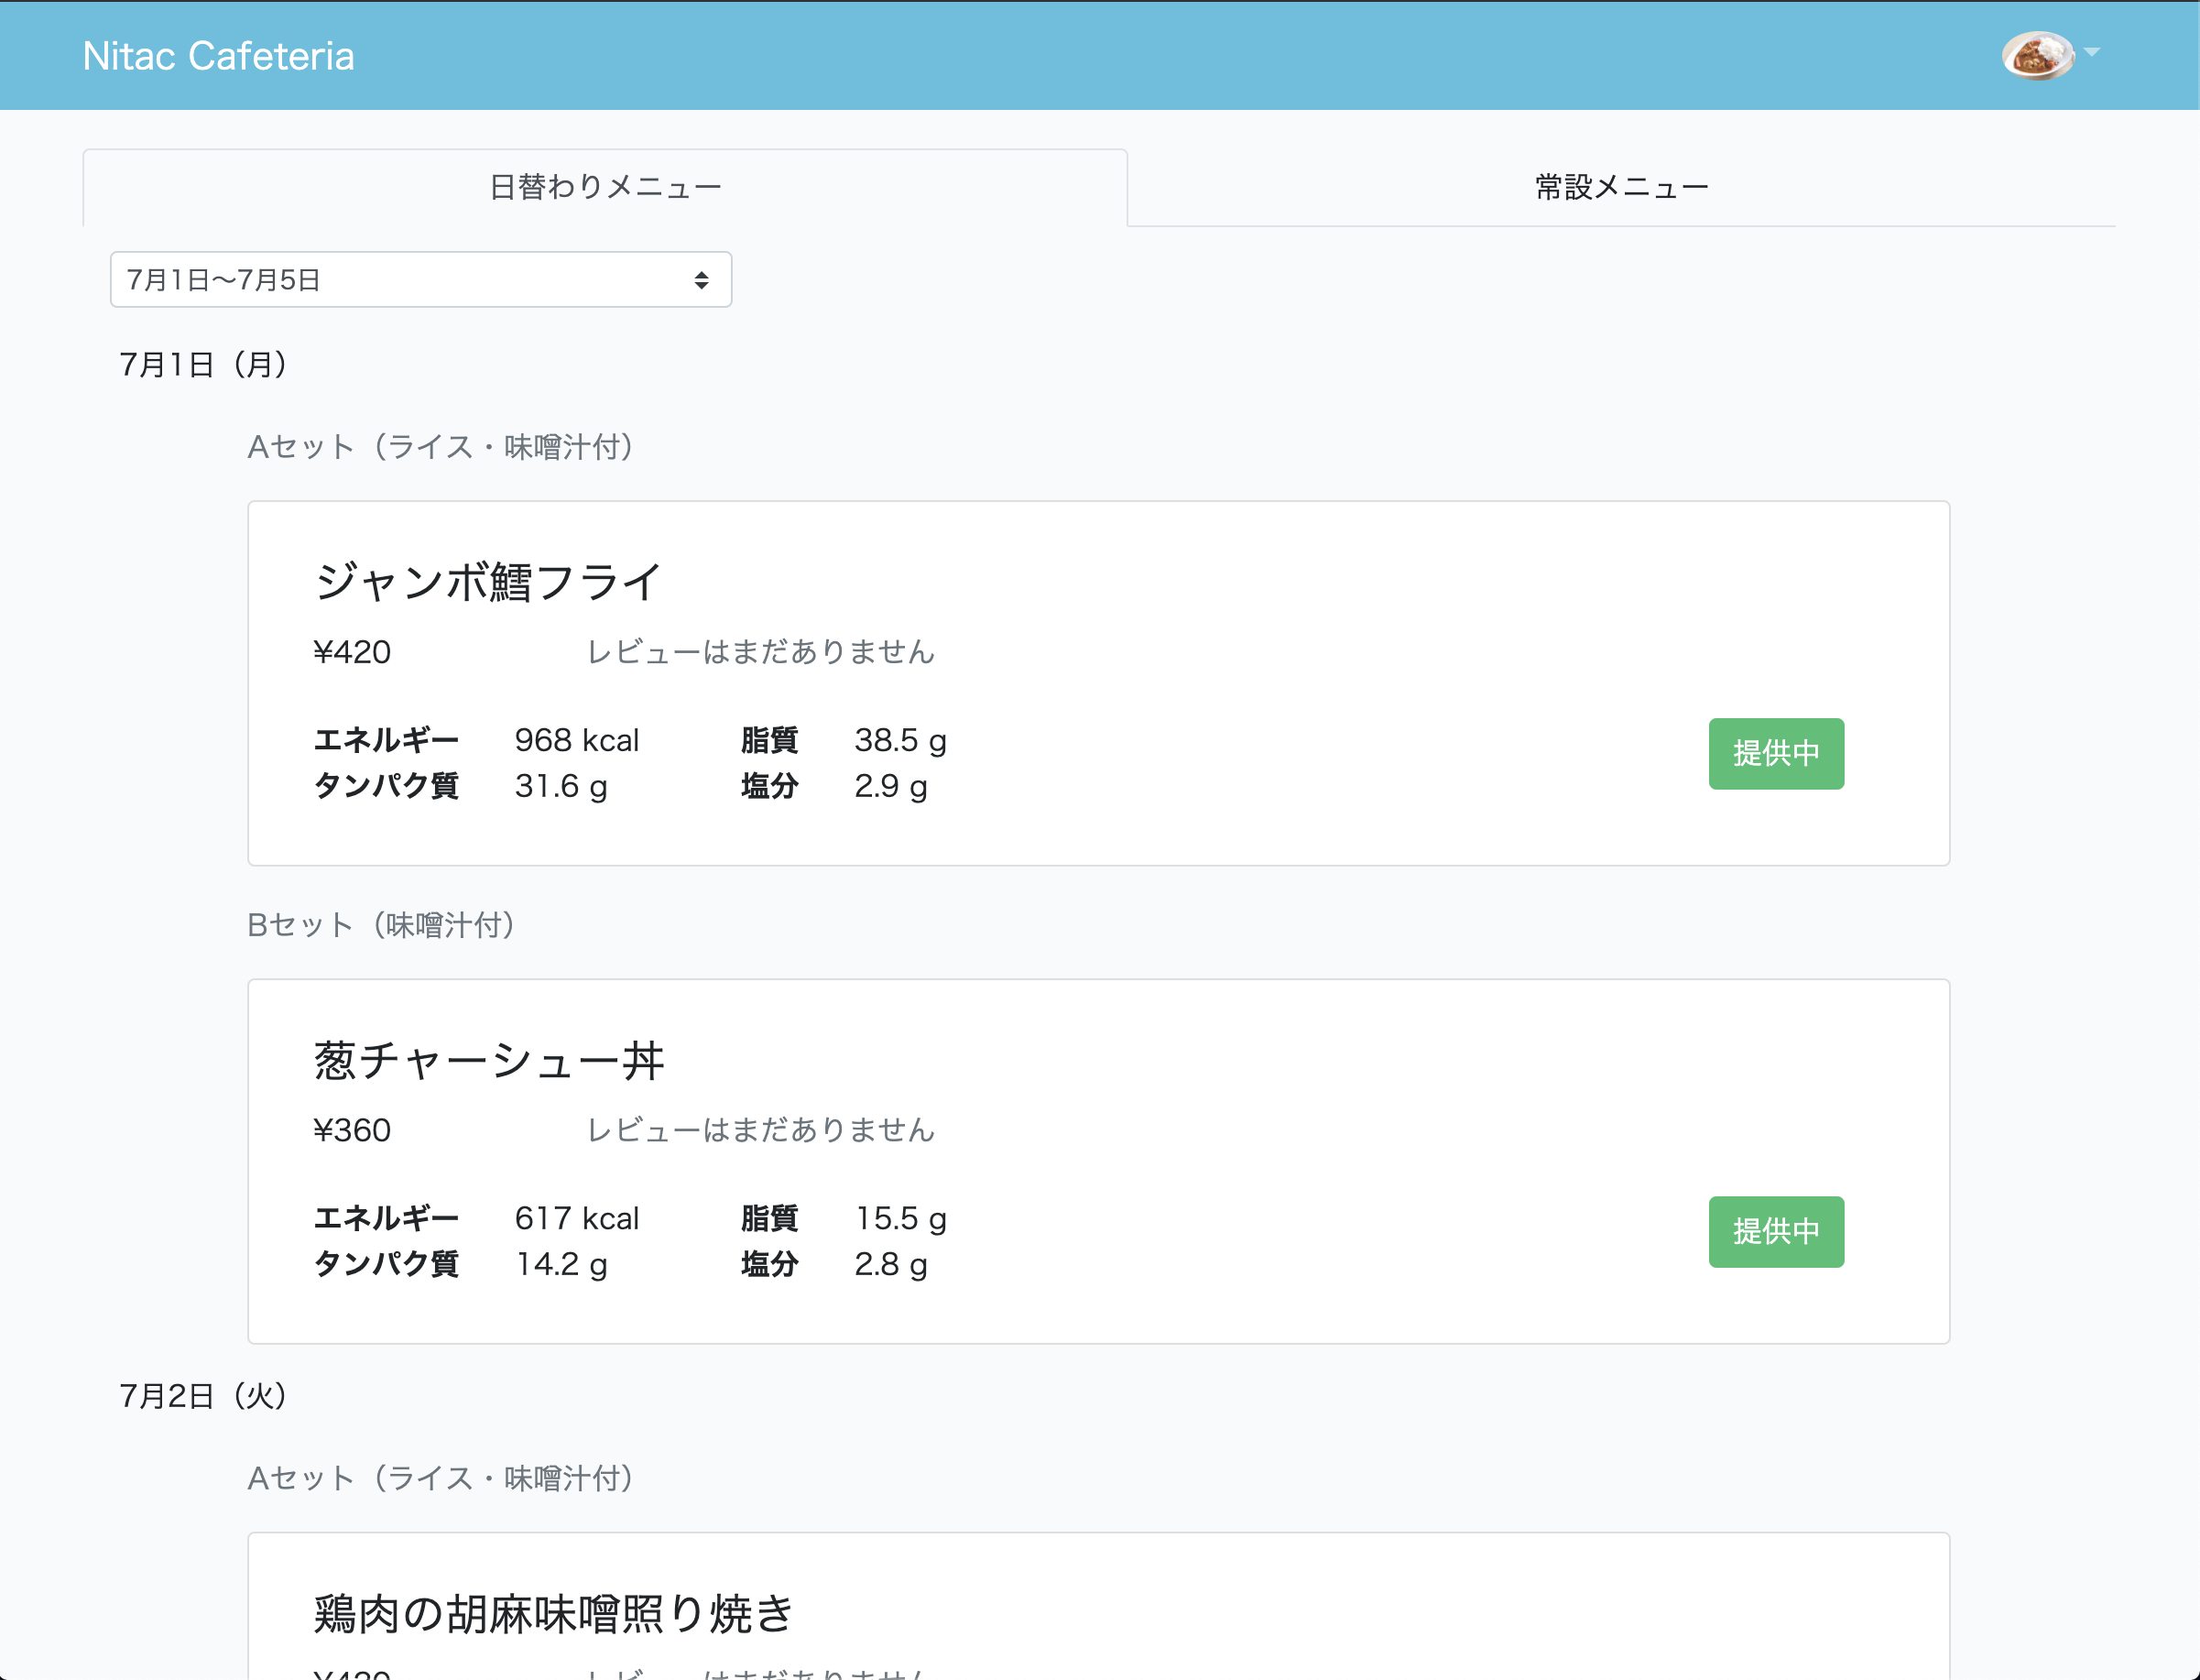
\includegraphics[scale = 0.225]{image/menu_admin.png}
	\caption{メニュー画面(管理者用)}
	\end{figure}
	管理者ログイン時の場合ユーザーログイン時とは異なり、お気に入り登録やレビューを投稿することはできません。提供中の状態の切り替えを行うことはできます。\\
	また右上のアイコンをタップするとドロップダウンが表示され、マイページ、管理者用ページ、メニュー検索、ログアウトが行えます。
	\newpage
\subsection{ドロップダウンの表示}
\begin{figure}[htbp]
	\centering
	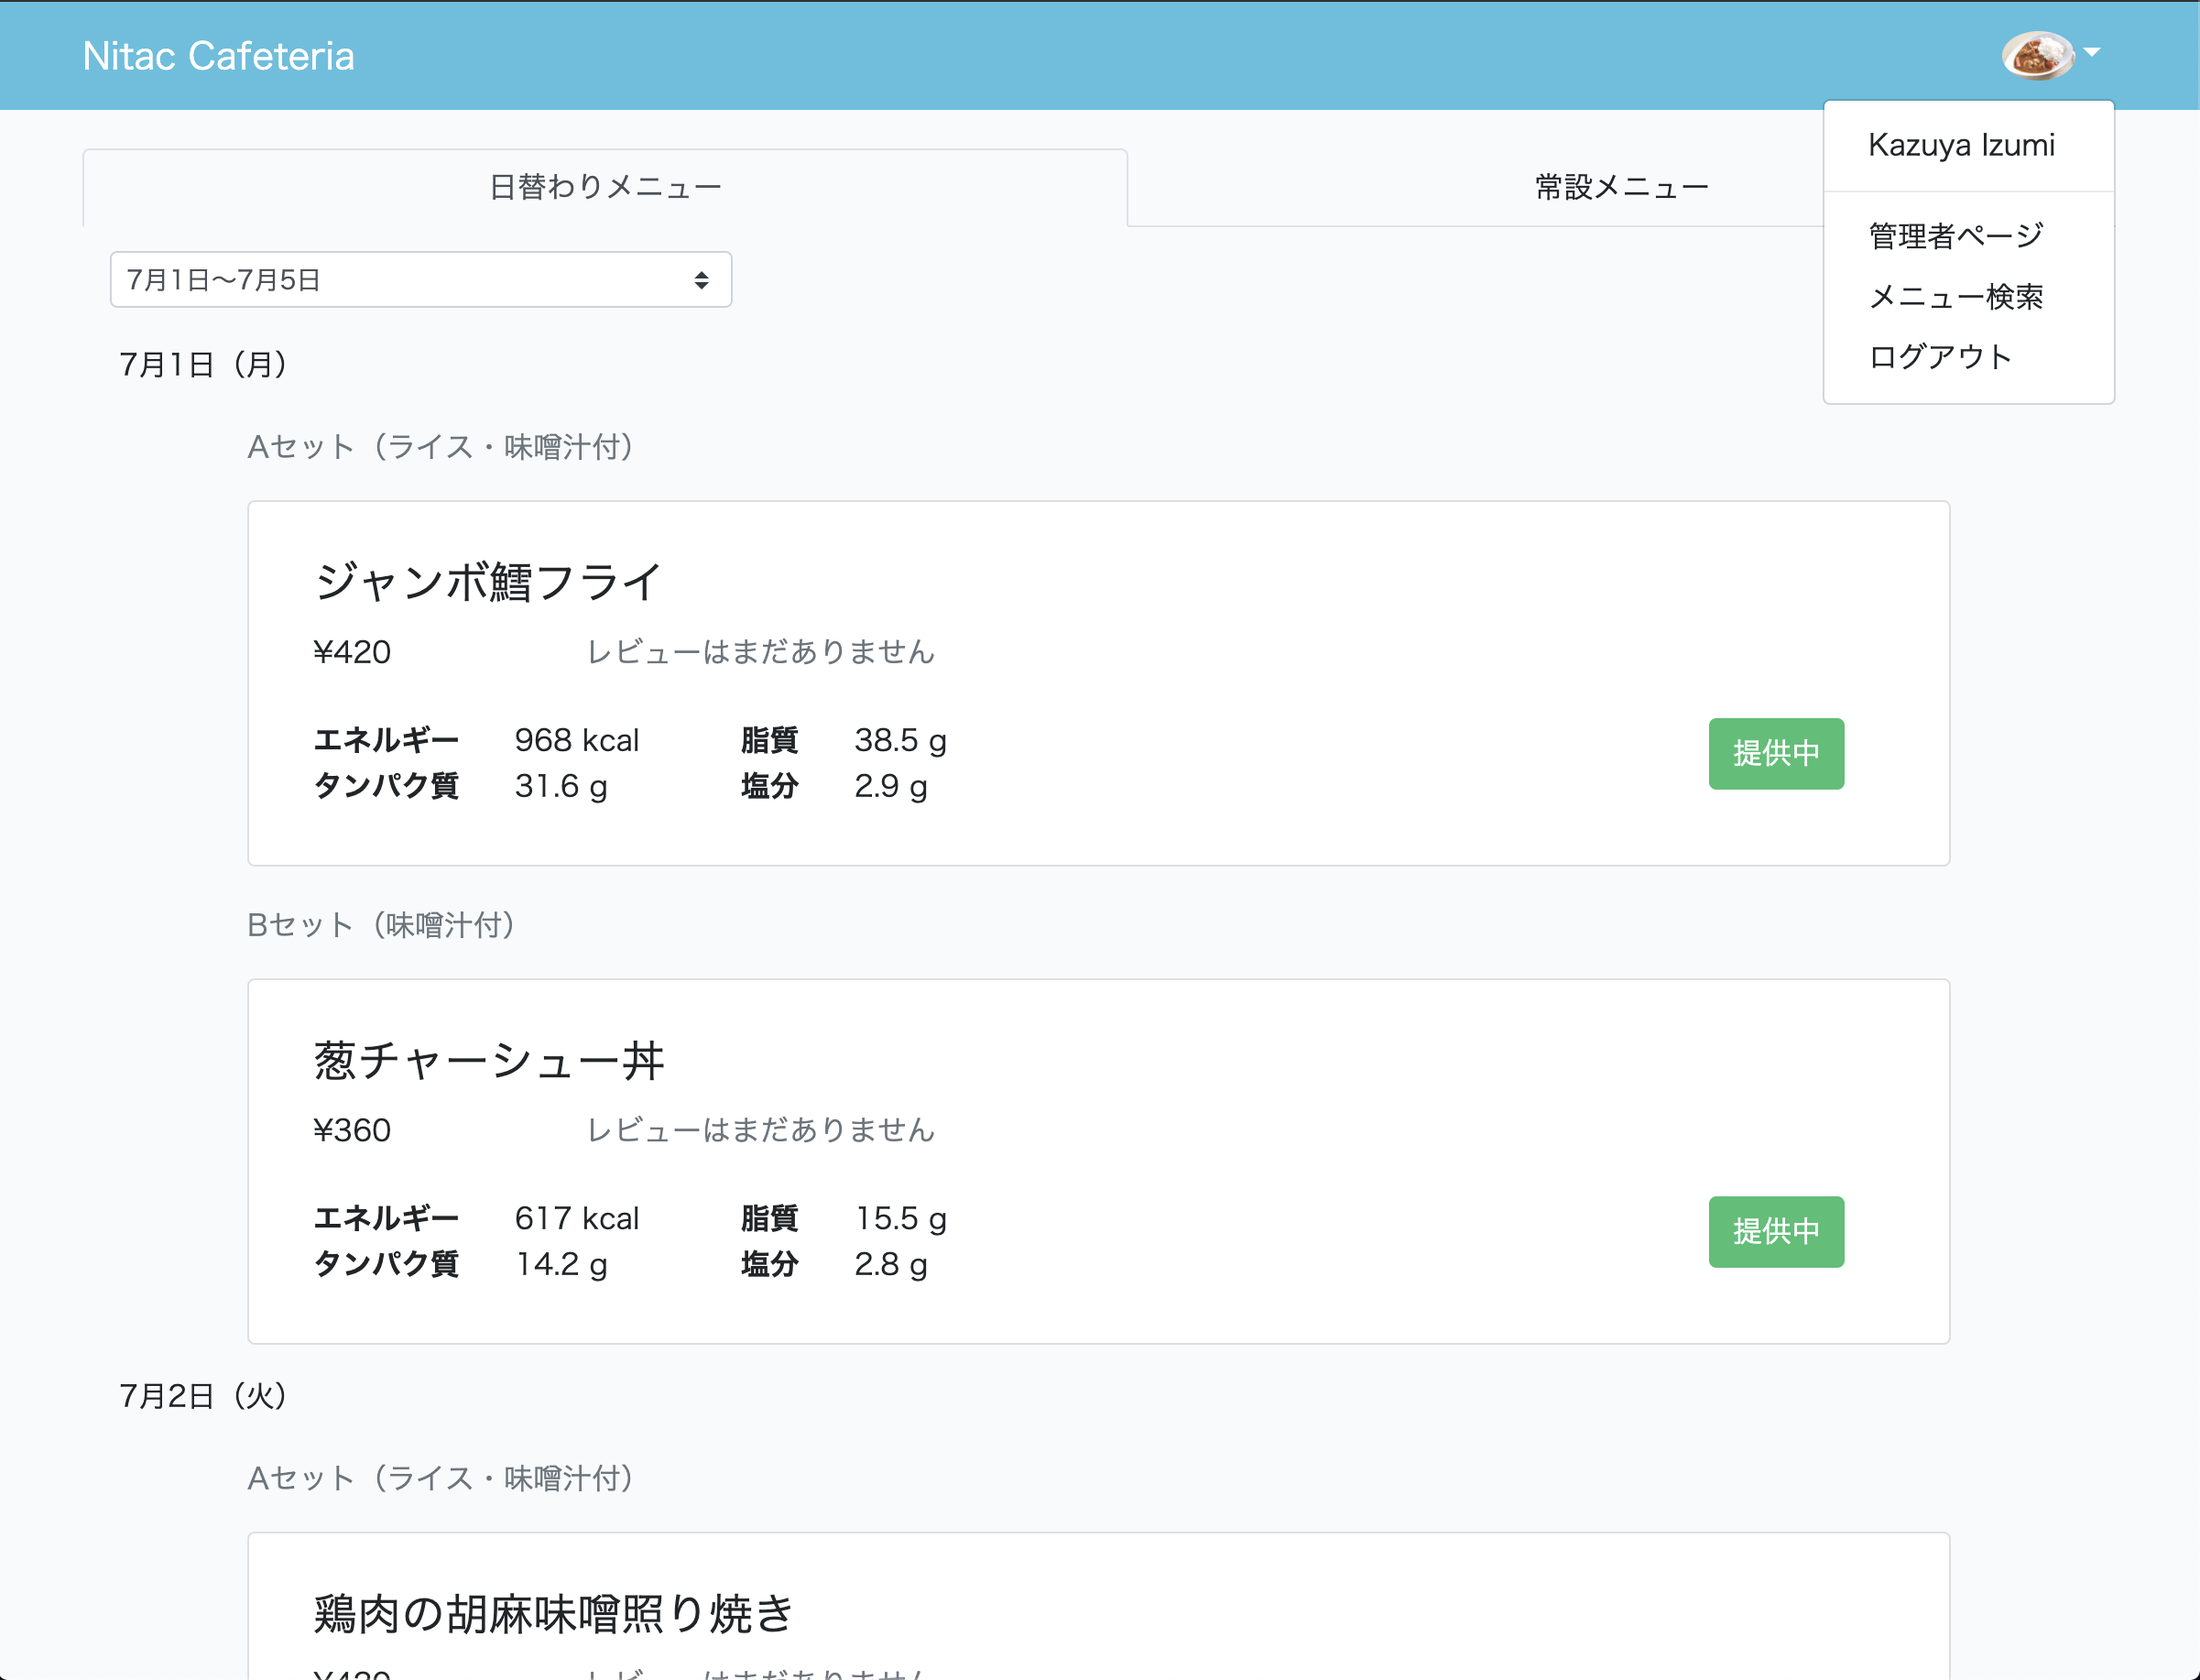
\includegraphics[scale = 0.225]{image/dropdown_admin.png}
	\caption{ドロップダウン画面(管理者用)}
	\end{figure}
	右上のアイコンをタップすると上の画面のようにドロップダウンが表示されます。\\
	ドロップダウンからマイページ、管理者用ページ(メニュー登録画面またはメニュー設定画面)、メニュー検索画面に遷移できます。\\
\newpage
\subsection{マイページ画面}
\begin{figure}[htbp]
	\centering
	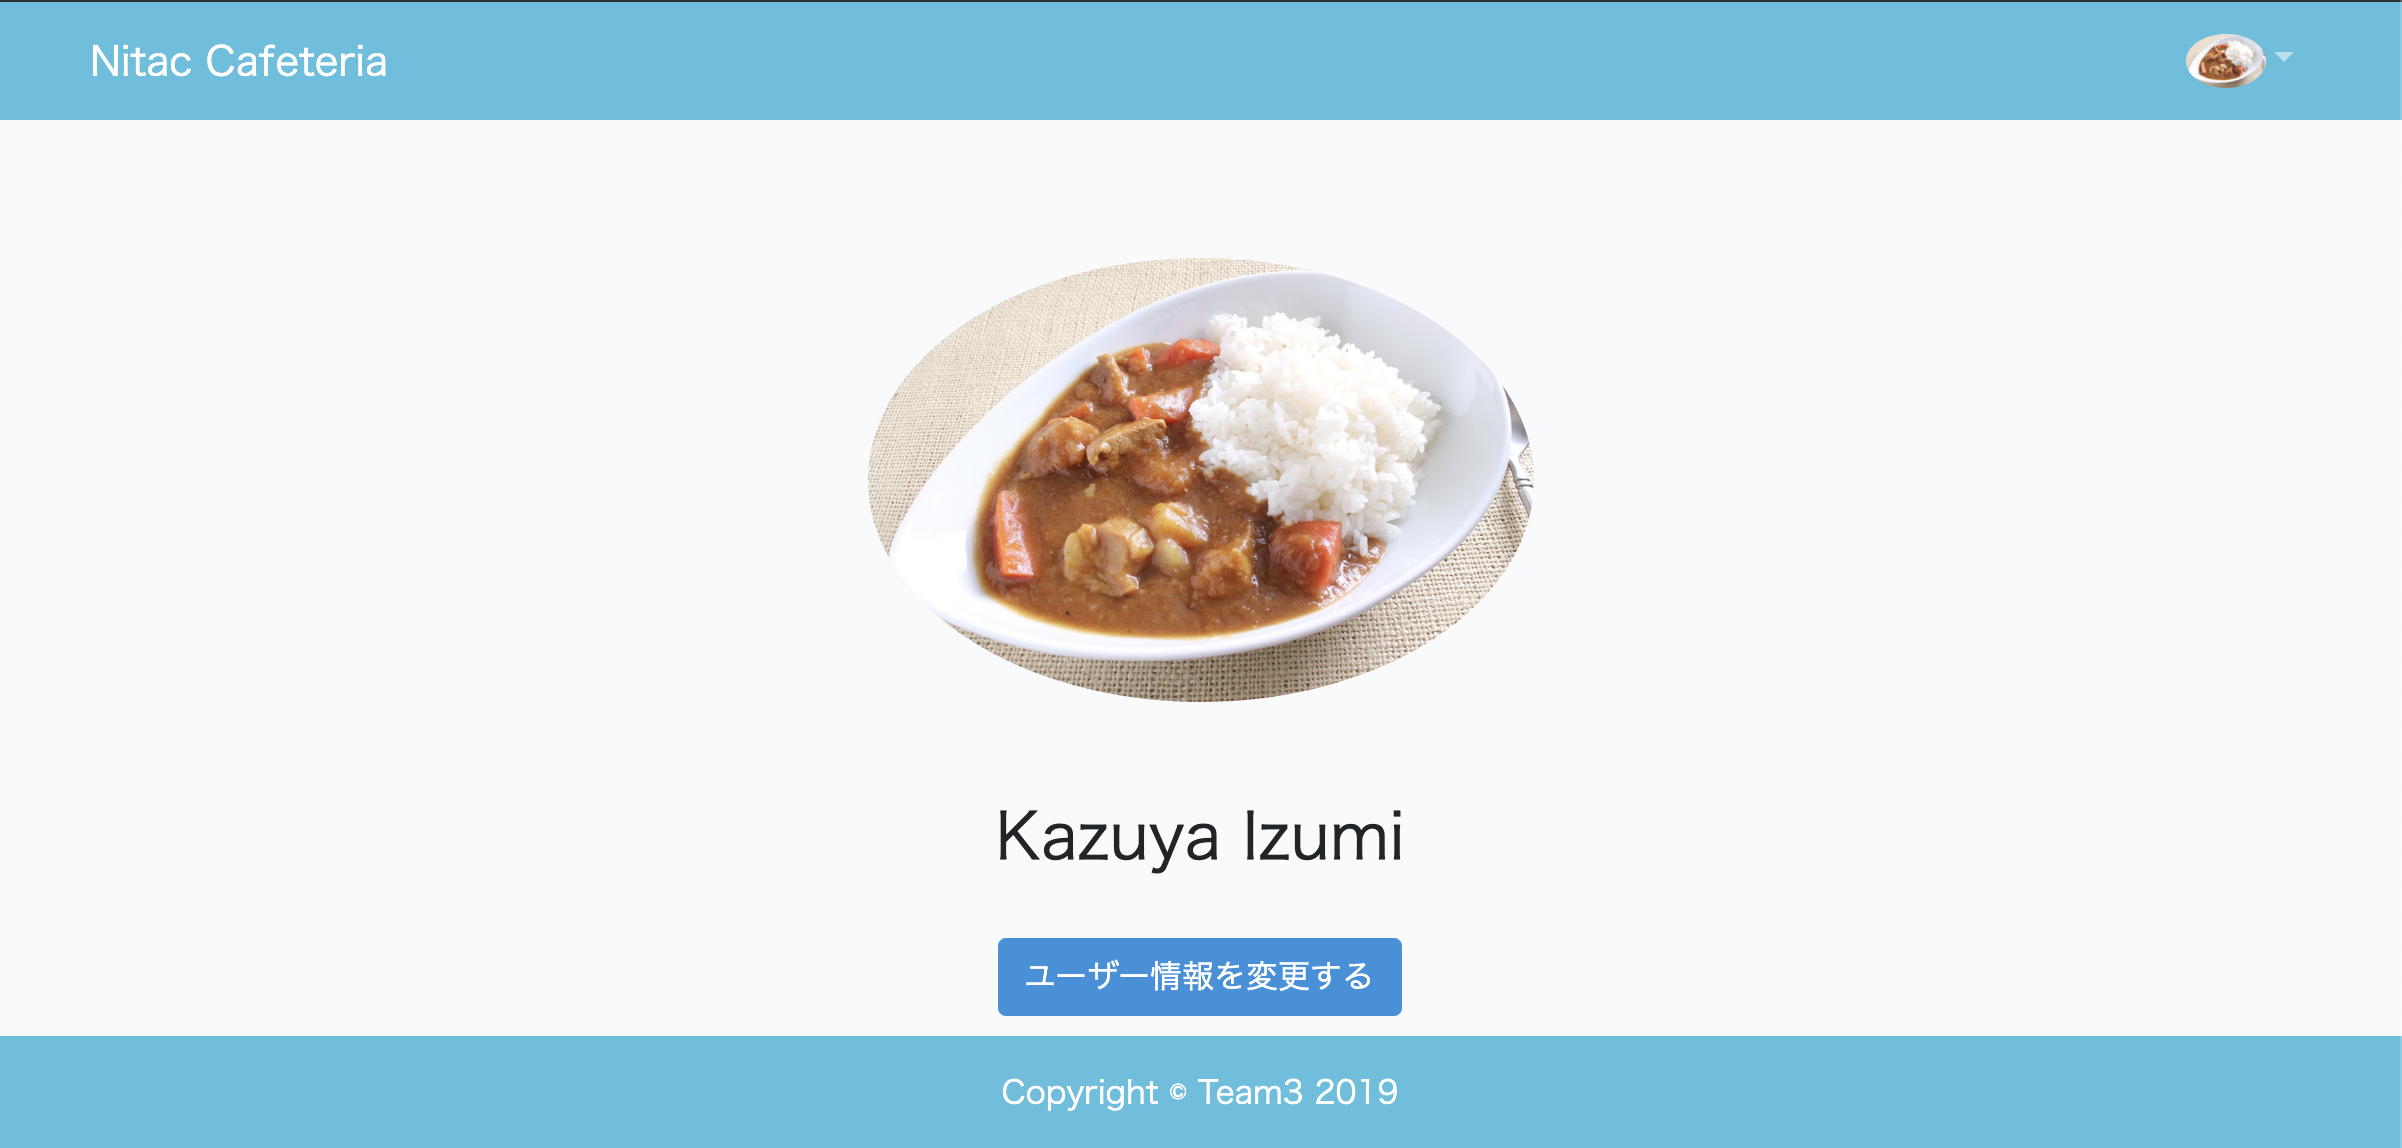
\includegraphics[scale = 0.225]{image/mypage_admin.png}
	\caption{マイページ画面(管理者用)}
	\end{figure}
	この画面ではユーザーログイン時と同様にユーザー情報変更画面への遷移をすることができます。
\subsection{メニュー登録画面}
\begin{figure}[htbp]
\centering
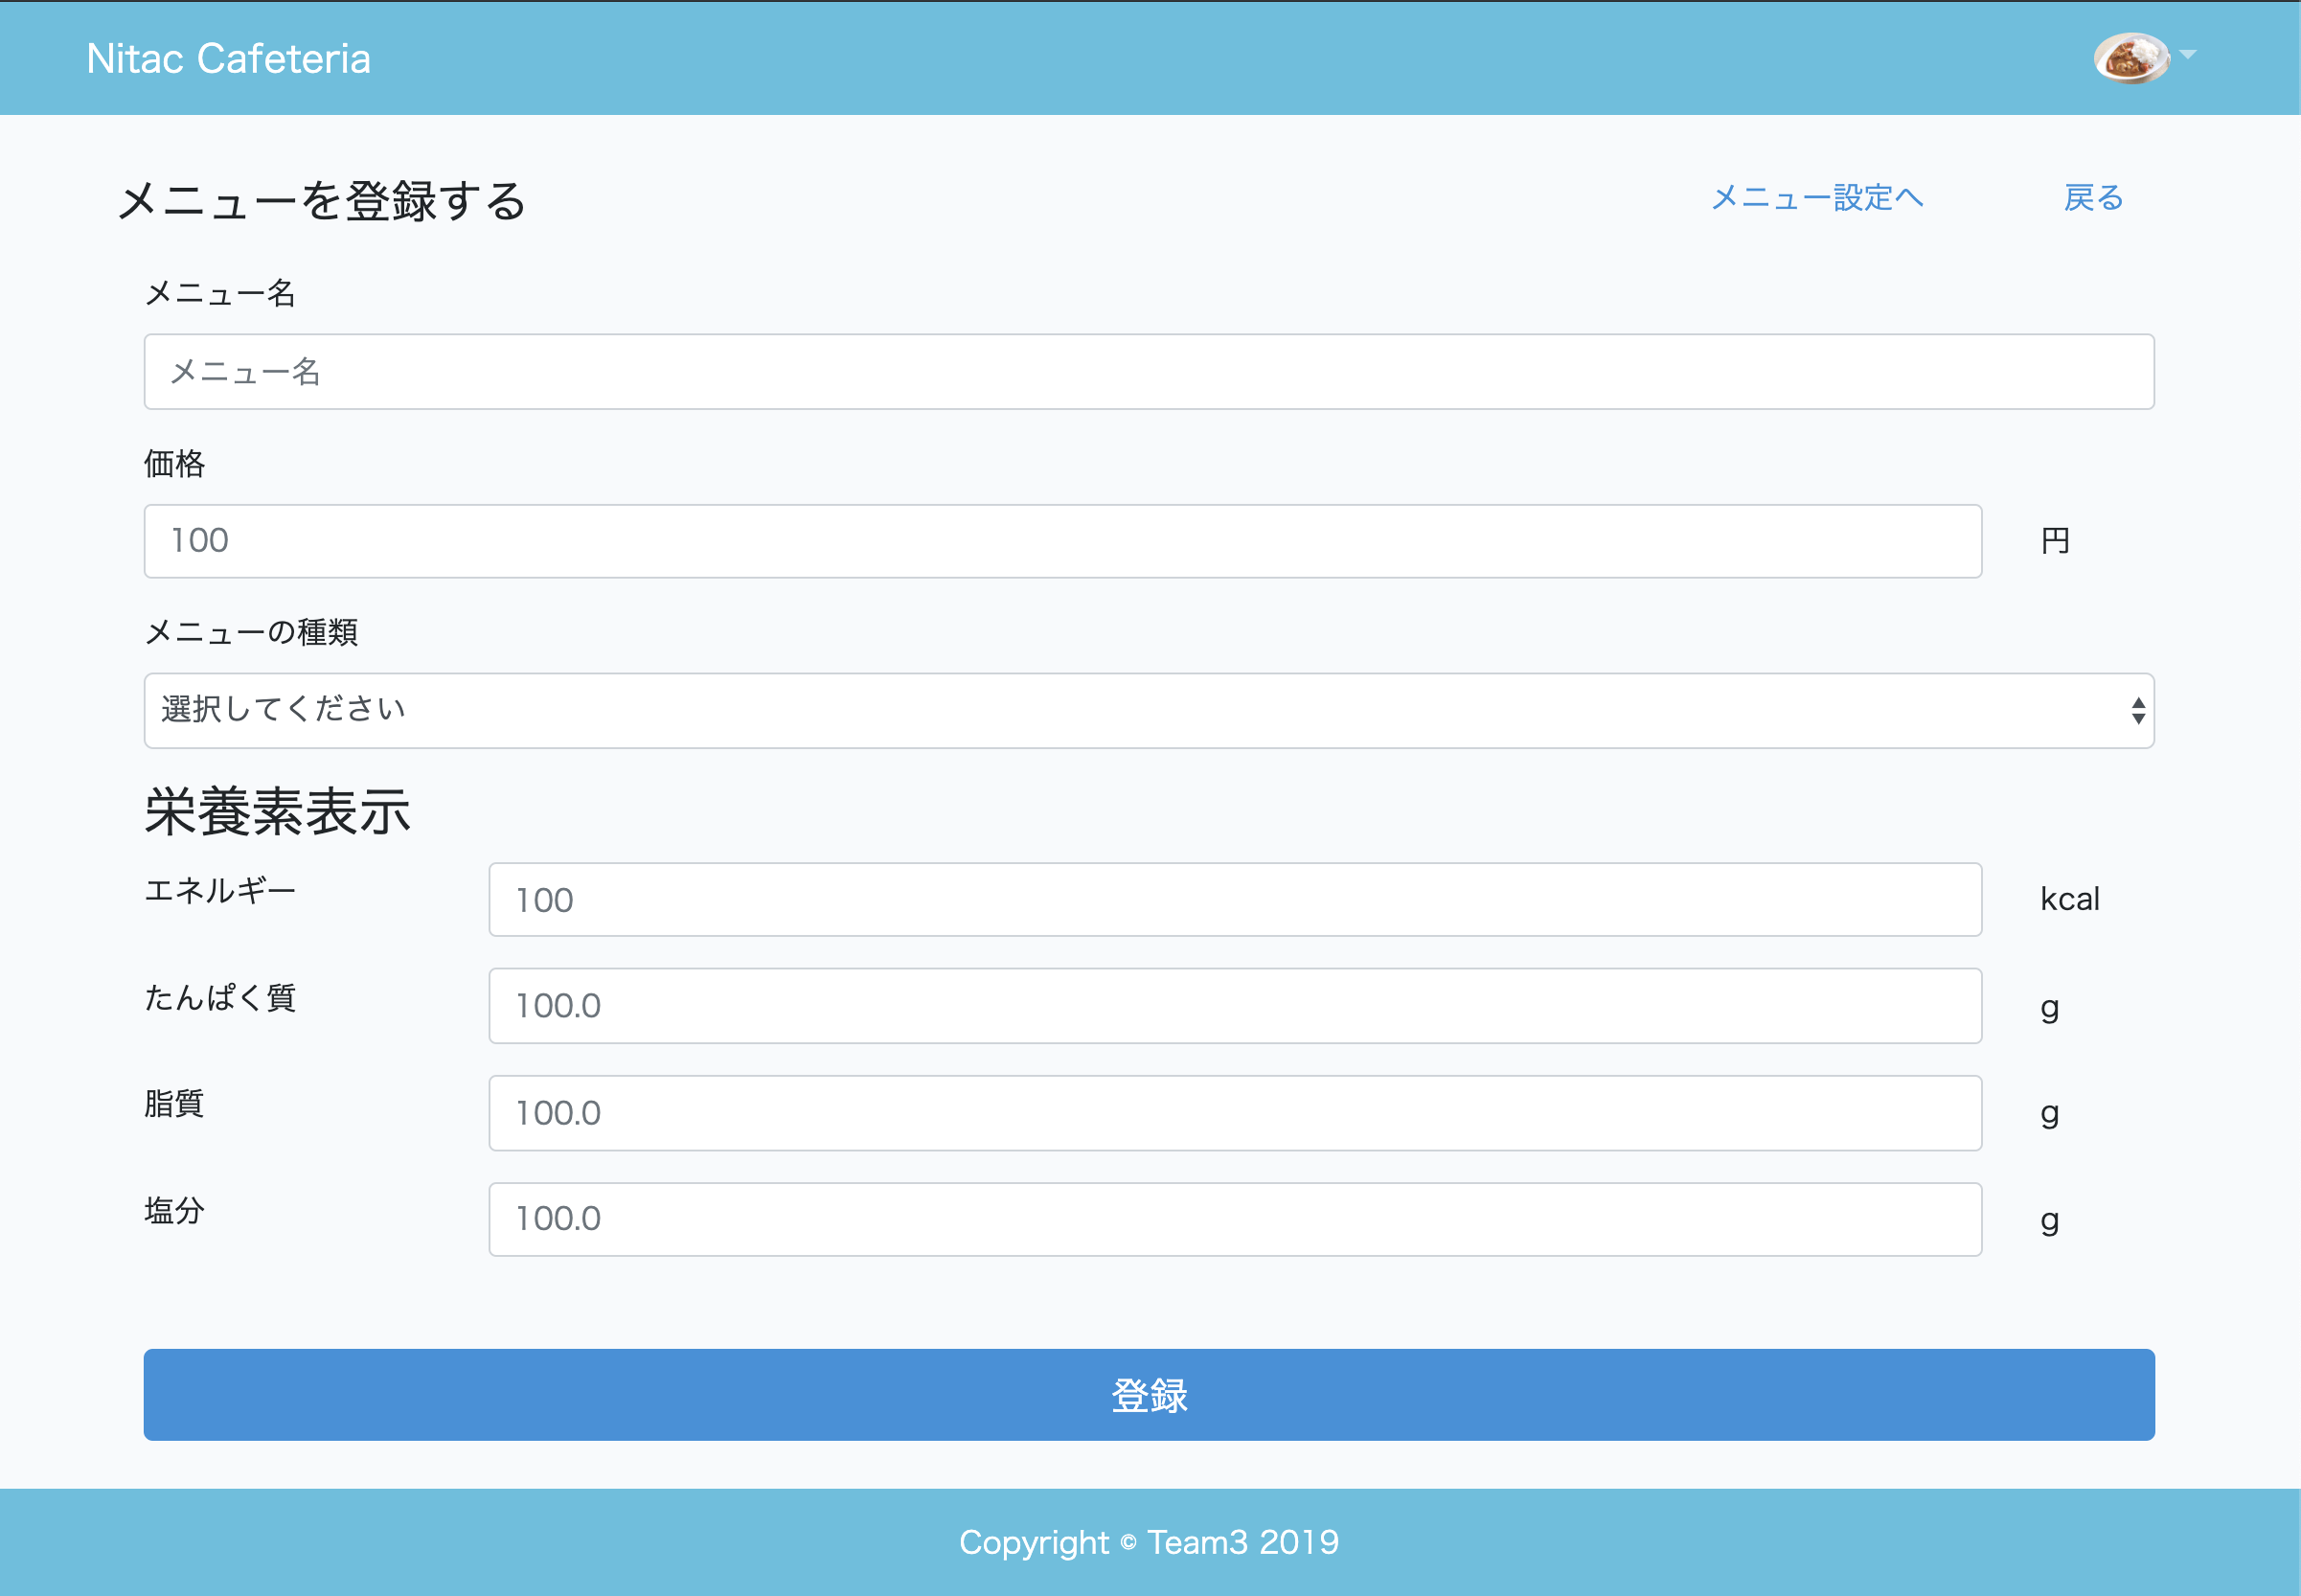
\includegraphics[scale = 0.225]{image/create_menu.png}
\caption{メニュー登録画面}
\end{figure}
この画面では、メニューの登録を行うことができます。\\
各項目を入力した後に、登録をタップすると登録が完了します。\\
登録したメニューを設定したい場合は、画面右上の「メニュー設定へ」をタップすることでメニュー設定画面に遷移することができます。
\newpage
\subsection{メニュー設定画面}
\begin{figure}[htbp]
\centering
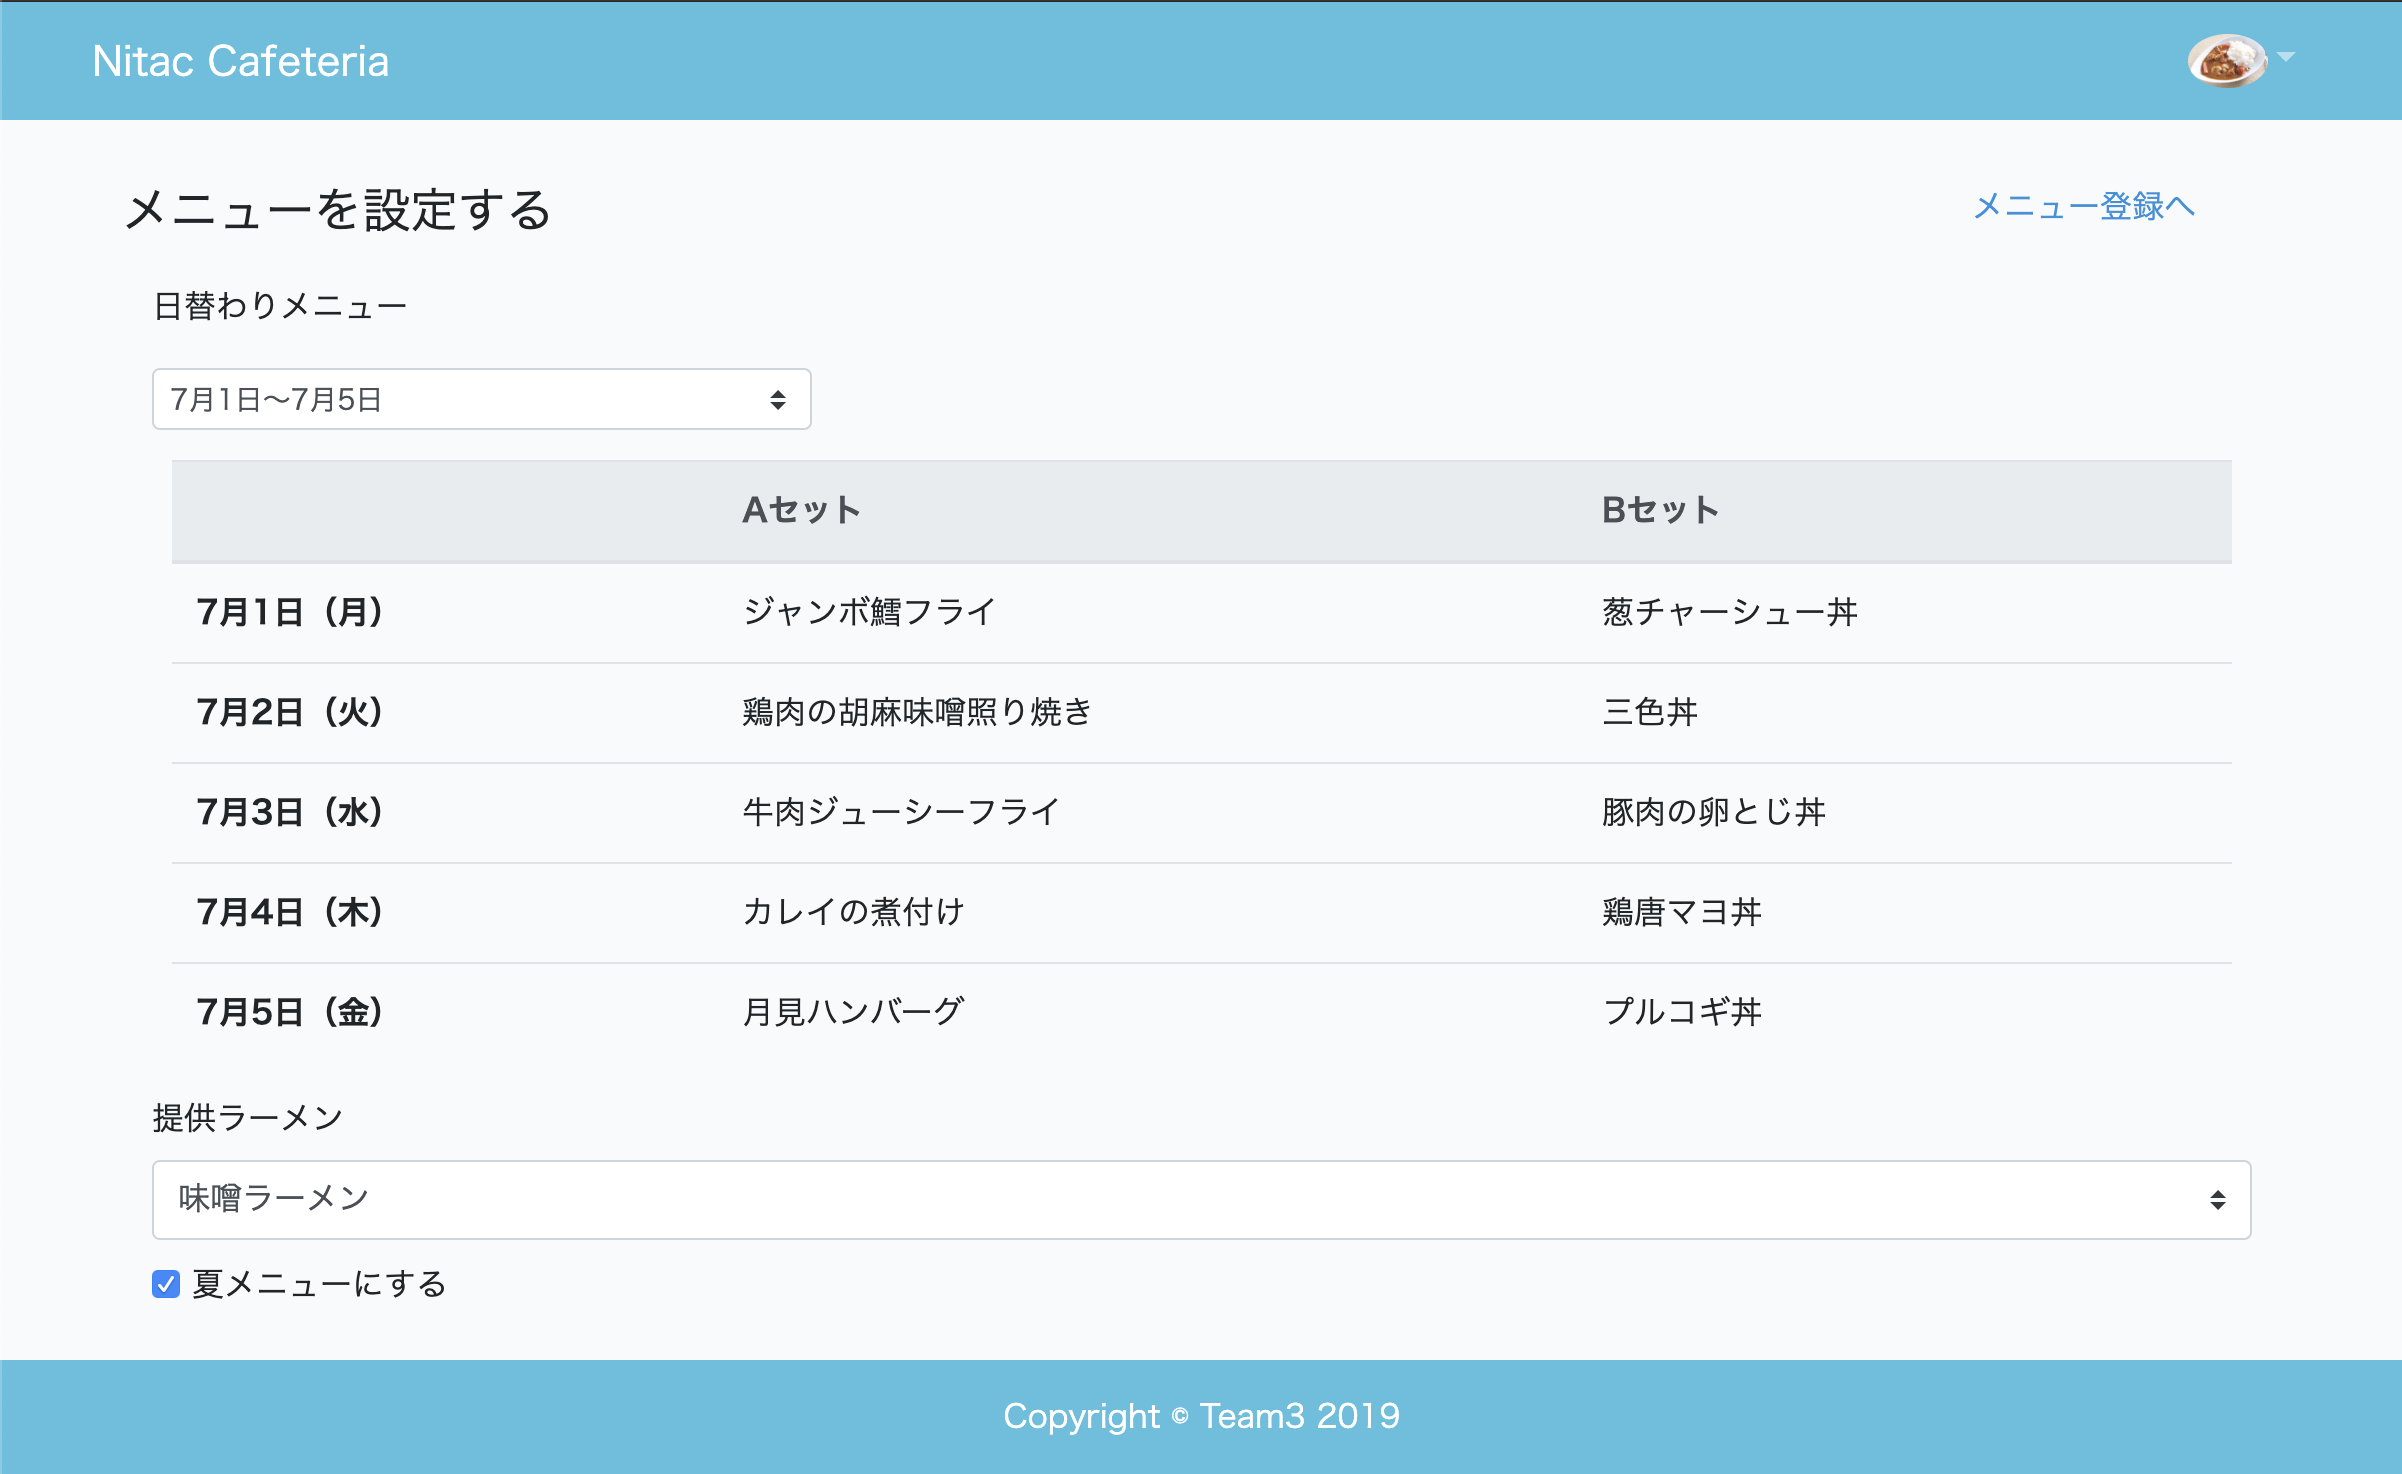
\includegraphics[scale = 0.225]{image/set_menu.png}
\caption{メニュー設定画面}
\end{figure}
この画面では、メニューの設定を行うことができます。\\
任意の場所をタップすると以下の画面が表示されるので、登録されたメニューの中から設定したいメニューを選択し、「変更する」をタップするとメニューの設定を行うことができます。
\begin{figure}[htbp]
\centering
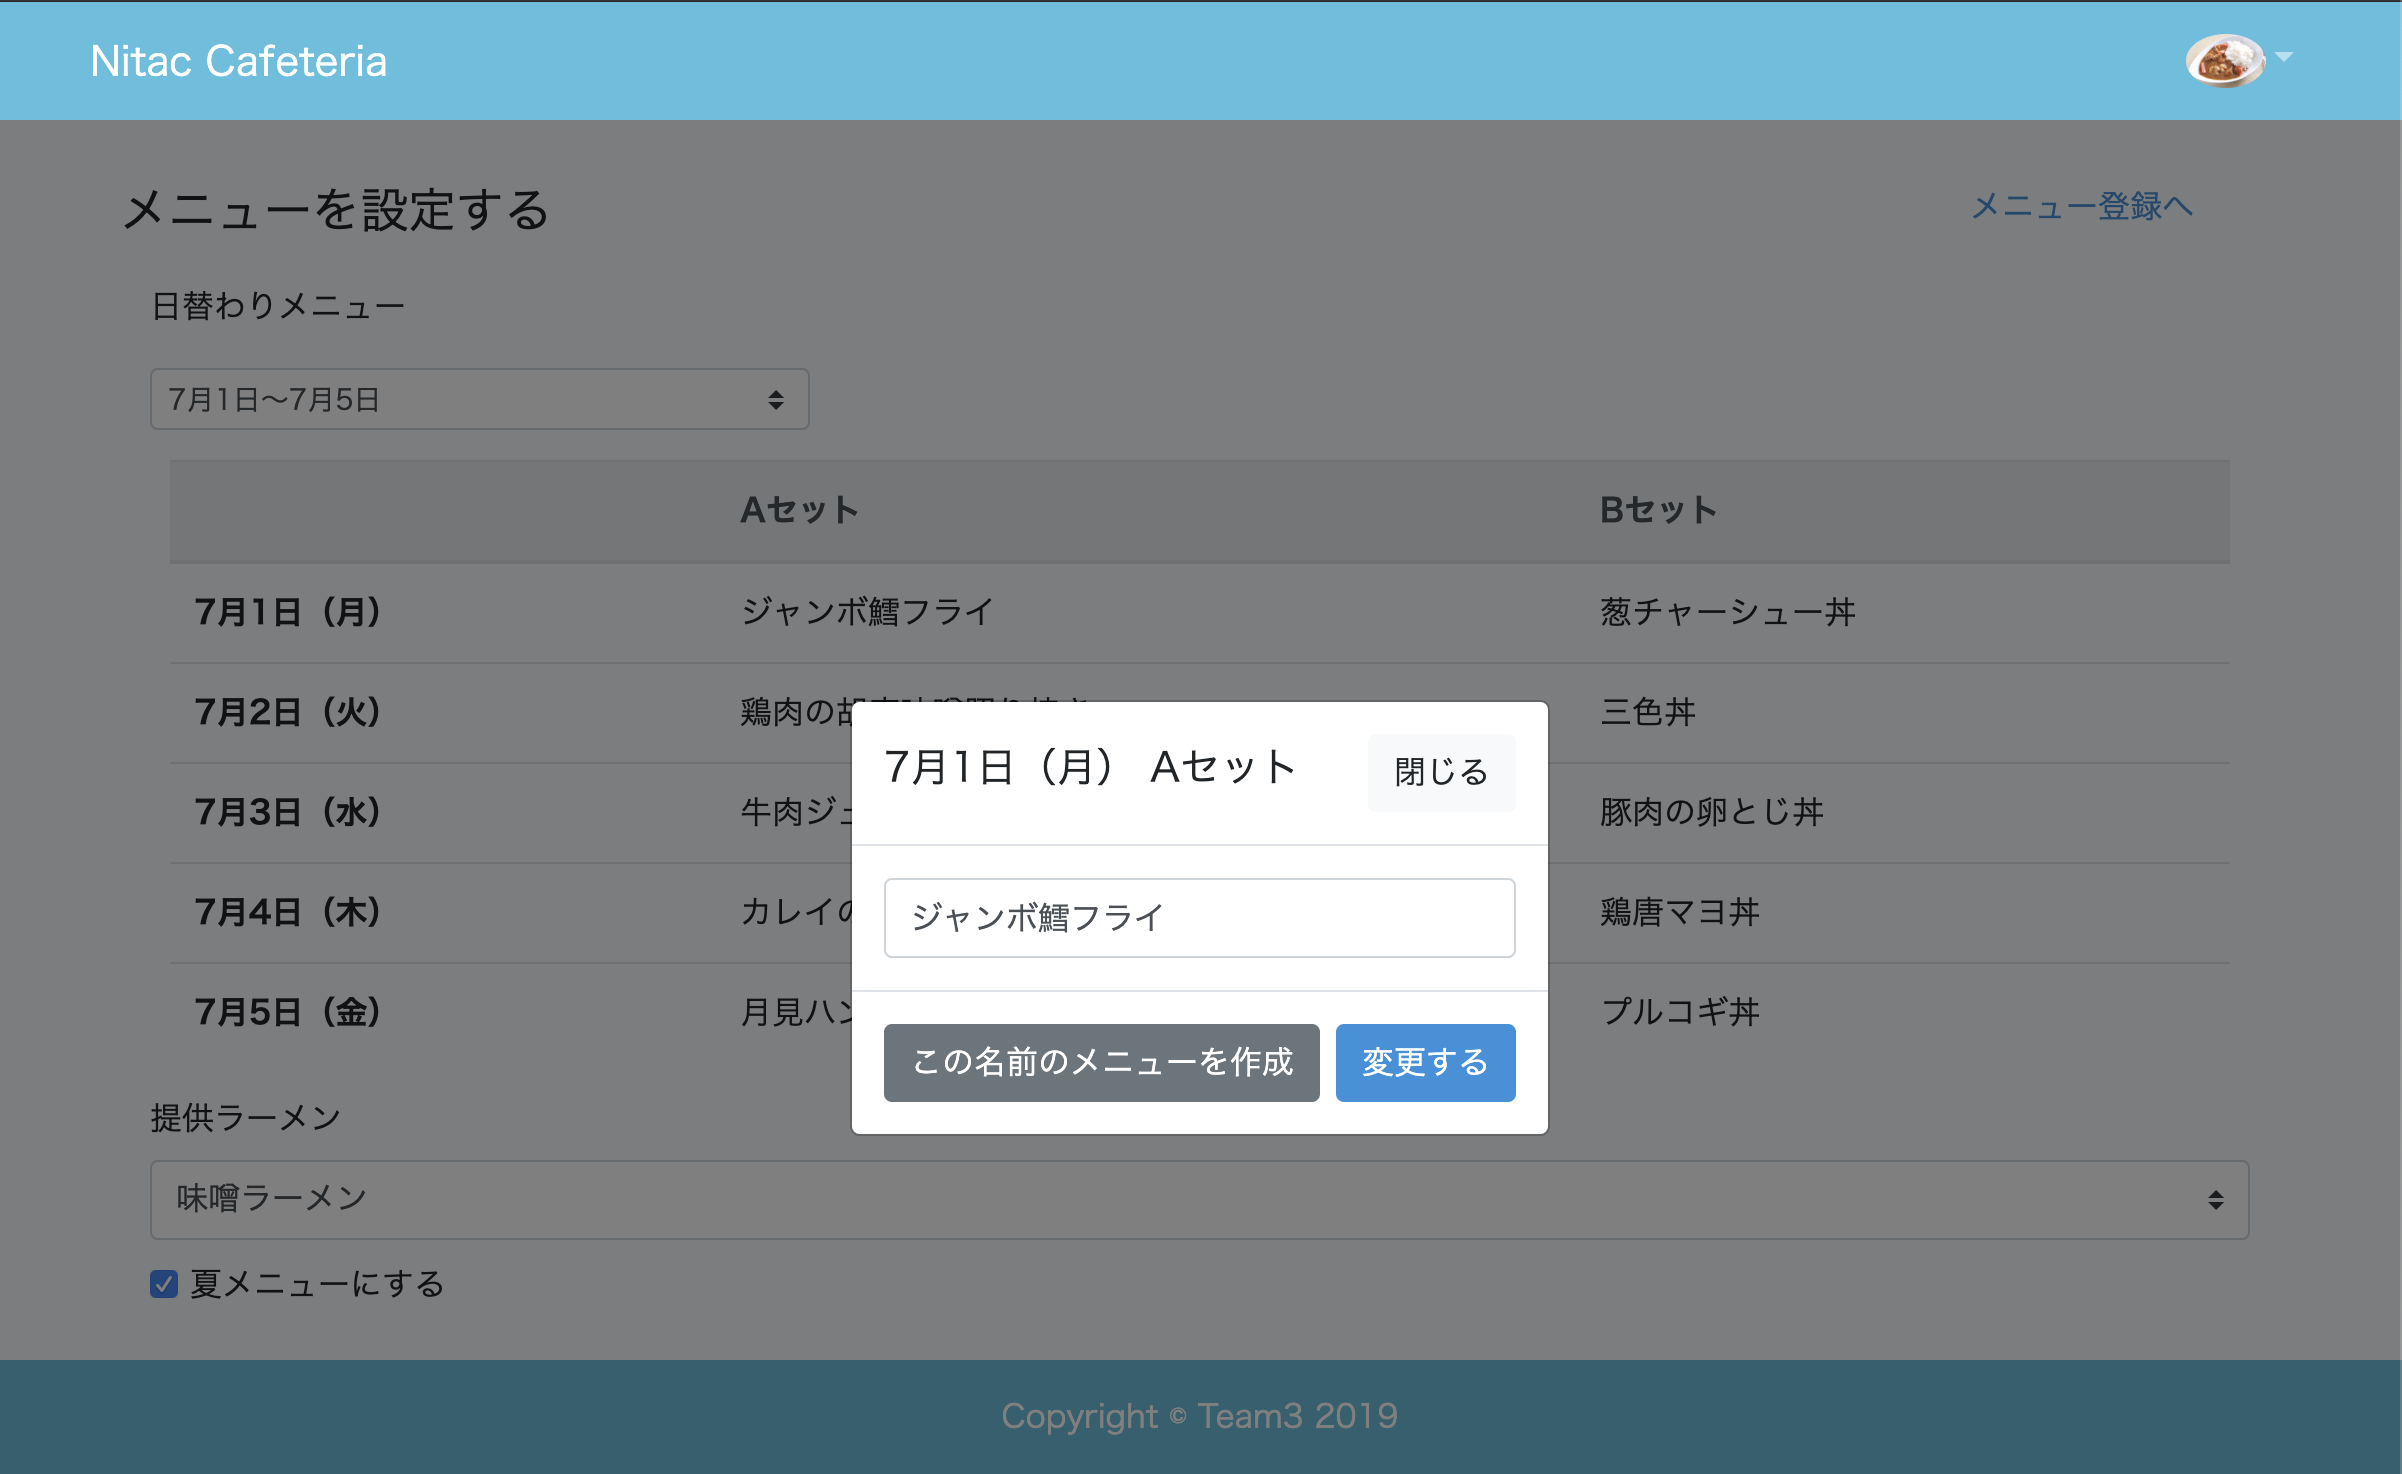
\includegraphics[scale = 0.225]{image/set_menu2.png}
\caption{メニュー設定画面}
\end{figure}
\newpage
\section{ログイン・ログアウト}
	\begin{figure}[htbp]
	\centering
	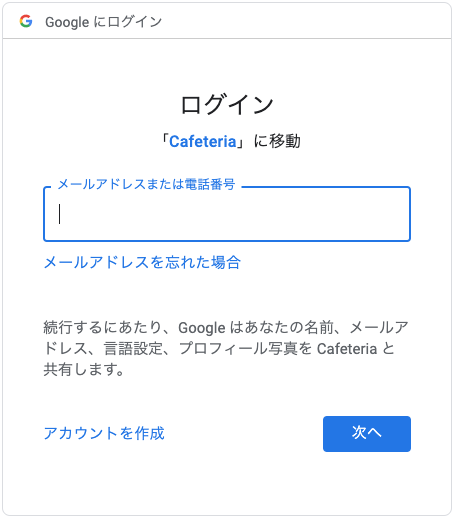
\includegraphics[scale = 0.35]{image/login.png}
	\caption{ログイン画面}
	\end{figure}
	画面右上のSign in with Googleをタップすると、ログイン画面に遷移します。\\
	ログインにはGoogleアカウントが必要なので、お持ちでない方はアカウントを作成して頂く必要があります。
	画面右上のアイコンをタップして、表示されたドロップダウンの中にある「ログアウト」をタップすると、ログアウトが完了します。
	\newpage
	\section{メニュー検索画面(ログイン時のみ)}
	\begin{figure}[htbp]
		\centering
		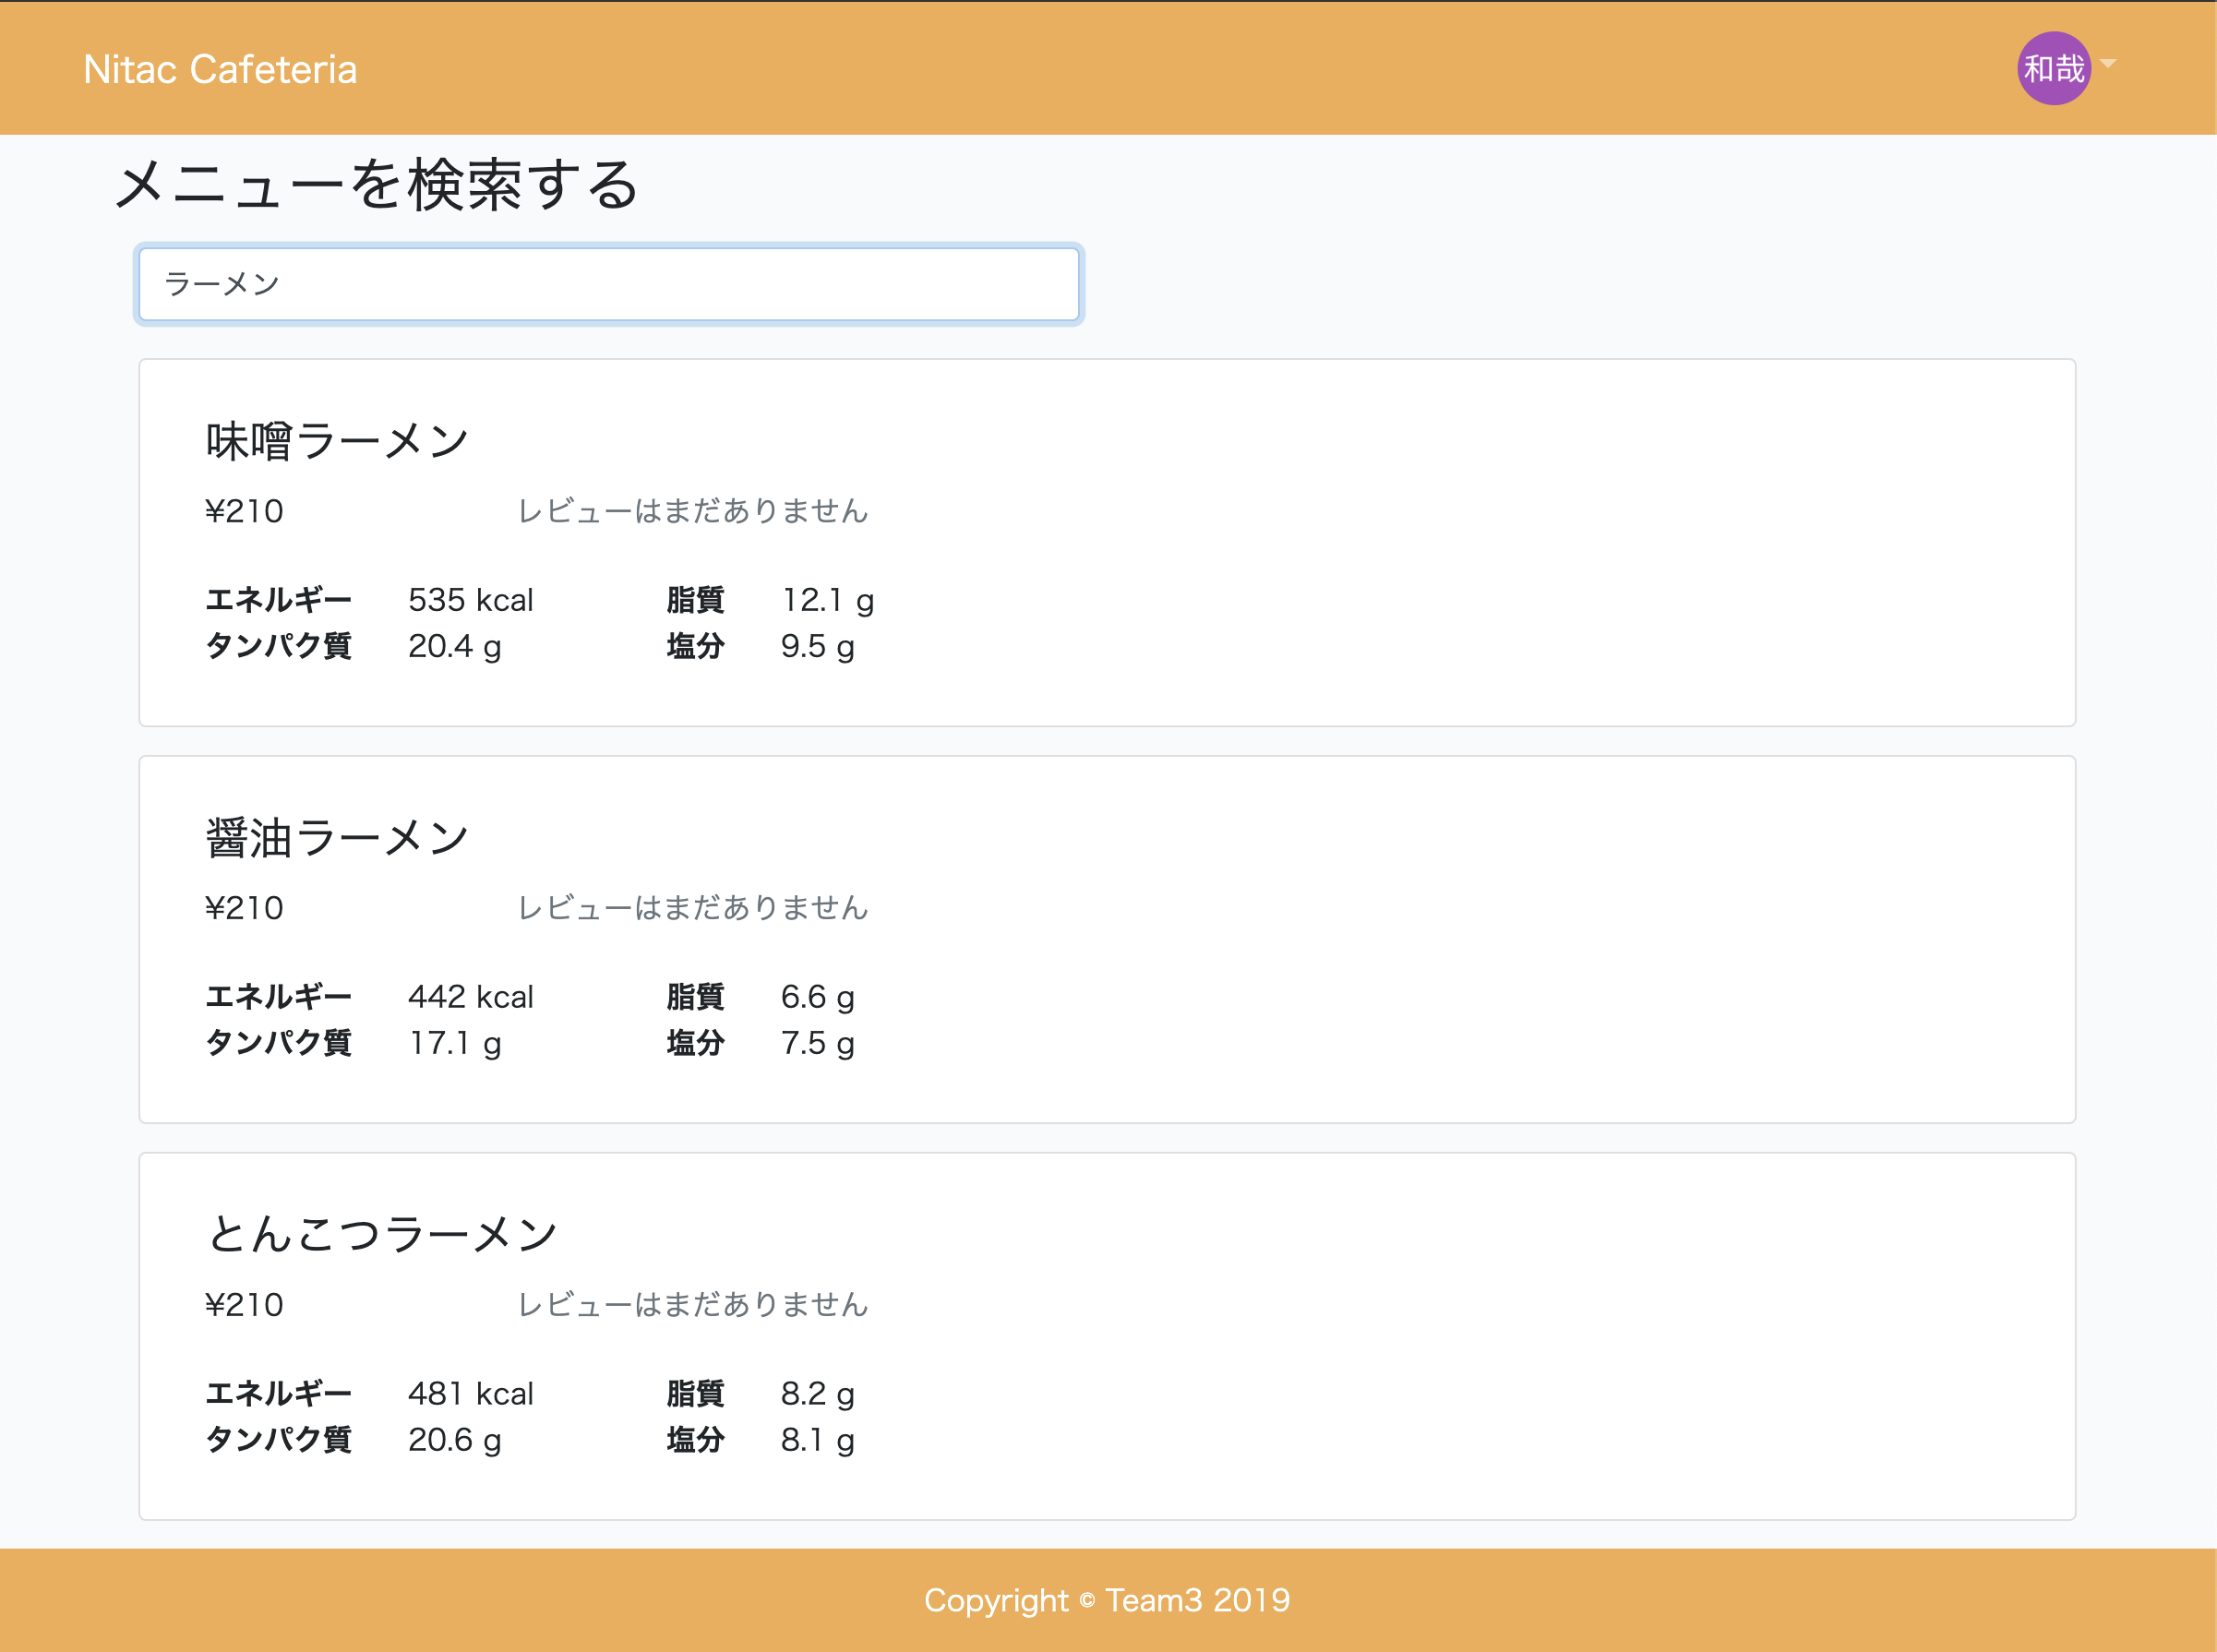
\includegraphics[scale = 0.225]{image/menu_search_ramen.png}
		\caption{メニュー検索画面}
		\end{figure}
		画面右上のアイコンをタップして、表示されたドロップダウンの中にある「メニュー検索」をタップするとメニュー検索画面に遷移することができます。\\
		上の画面は「ラーメン」と検索したときの例です。		
\end{document}
